% Options for packages loaded elsewhere
\PassOptionsToPackage{unicode}{hyperref}
\PassOptionsToPackage{hyphens}{url}
\documentclass[
]{article}
\usepackage{xcolor}
\usepackage[margin=1in]{geometry}
\usepackage{amsmath,amssymb}
\setcounter{secnumdepth}{5}
\usepackage{iftex}
\ifPDFTeX
  \usepackage[T1]{fontenc}
  \usepackage[utf8]{inputenc}
  \usepackage{textcomp} % provide euro and other symbols
\else % if luatex or xetex
  \usepackage{unicode-math} % this also loads fontspec
  \defaultfontfeatures{Scale=MatchLowercase}
  \defaultfontfeatures[\rmfamily]{Ligatures=TeX,Scale=1}
\fi
\usepackage{lmodern}
\ifPDFTeX\else
  % xetex/luatex font selection
\fi
% Use upquote if available, for straight quotes in verbatim environments
\IfFileExists{upquote.sty}{\usepackage{upquote}}{}
\IfFileExists{microtype.sty}{% use microtype if available
  \usepackage[]{microtype}
  \UseMicrotypeSet[protrusion]{basicmath} % disable protrusion for tt fonts
}{}
\makeatletter
\@ifundefined{KOMAClassName}{% if non-KOMA class
  \IfFileExists{parskip.sty}{%
    \usepackage{parskip}
  }{% else
    \setlength{\parindent}{0pt}
    \setlength{\parskip}{6pt plus 2pt minus 1pt}}
}{% if KOMA class
  \KOMAoptions{parskip=half}}
\makeatother
\usepackage{color}
\usepackage{fancyvrb}
\newcommand{\VerbBar}{|}
\newcommand{\VERB}{\Verb[commandchars=\\\{\}]}
\DefineVerbatimEnvironment{Highlighting}{Verbatim}{commandchars=\\\{\}}
% Add ',fontsize=\small' for more characters per line
\usepackage{framed}
\definecolor{shadecolor}{RGB}{248,248,248}
\newenvironment{Shaded}{\begin{snugshade}}{\end{snugshade}}
\newcommand{\AlertTok}[1]{\textcolor[rgb]{0.94,0.16,0.16}{#1}}
\newcommand{\AnnotationTok}[1]{\textcolor[rgb]{0.56,0.35,0.01}{\textbf{\textit{#1}}}}
\newcommand{\AttributeTok}[1]{\textcolor[rgb]{0.13,0.29,0.53}{#1}}
\newcommand{\BaseNTok}[1]{\textcolor[rgb]{0.00,0.00,0.81}{#1}}
\newcommand{\BuiltInTok}[1]{#1}
\newcommand{\CharTok}[1]{\textcolor[rgb]{0.31,0.60,0.02}{#1}}
\newcommand{\CommentTok}[1]{\textcolor[rgb]{0.56,0.35,0.01}{\textit{#1}}}
\newcommand{\CommentVarTok}[1]{\textcolor[rgb]{0.56,0.35,0.01}{\textbf{\textit{#1}}}}
\newcommand{\ConstantTok}[1]{\textcolor[rgb]{0.56,0.35,0.01}{#1}}
\newcommand{\ControlFlowTok}[1]{\textcolor[rgb]{0.13,0.29,0.53}{\textbf{#1}}}
\newcommand{\DataTypeTok}[1]{\textcolor[rgb]{0.13,0.29,0.53}{#1}}
\newcommand{\DecValTok}[1]{\textcolor[rgb]{0.00,0.00,0.81}{#1}}
\newcommand{\DocumentationTok}[1]{\textcolor[rgb]{0.56,0.35,0.01}{\textbf{\textit{#1}}}}
\newcommand{\ErrorTok}[1]{\textcolor[rgb]{0.64,0.00,0.00}{\textbf{#1}}}
\newcommand{\ExtensionTok}[1]{#1}
\newcommand{\FloatTok}[1]{\textcolor[rgb]{0.00,0.00,0.81}{#1}}
\newcommand{\FunctionTok}[1]{\textcolor[rgb]{0.13,0.29,0.53}{\textbf{#1}}}
\newcommand{\ImportTok}[1]{#1}
\newcommand{\InformationTok}[1]{\textcolor[rgb]{0.56,0.35,0.01}{\textbf{\textit{#1}}}}
\newcommand{\KeywordTok}[1]{\textcolor[rgb]{0.13,0.29,0.53}{\textbf{#1}}}
\newcommand{\NormalTok}[1]{#1}
\newcommand{\OperatorTok}[1]{\textcolor[rgb]{0.81,0.36,0.00}{\textbf{#1}}}
\newcommand{\OtherTok}[1]{\textcolor[rgb]{0.56,0.35,0.01}{#1}}
\newcommand{\PreprocessorTok}[1]{\textcolor[rgb]{0.56,0.35,0.01}{\textit{#1}}}
\newcommand{\RegionMarkerTok}[1]{#1}
\newcommand{\SpecialCharTok}[1]{\textcolor[rgb]{0.81,0.36,0.00}{\textbf{#1}}}
\newcommand{\SpecialStringTok}[1]{\textcolor[rgb]{0.31,0.60,0.02}{#1}}
\newcommand{\StringTok}[1]{\textcolor[rgb]{0.31,0.60,0.02}{#1}}
\newcommand{\VariableTok}[1]{\textcolor[rgb]{0.00,0.00,0.00}{#1}}
\newcommand{\VerbatimStringTok}[1]{\textcolor[rgb]{0.31,0.60,0.02}{#1}}
\newcommand{\WarningTok}[1]{\textcolor[rgb]{0.56,0.35,0.01}{\textbf{\textit{#1}}}}
\usepackage{longtable,booktabs,array}
\usepackage{calc} % for calculating minipage widths
% Correct order of tables after \paragraph or \subparagraph
\usepackage{etoolbox}
\makeatletter
\patchcmd\longtable{\par}{\if@noskipsec\mbox{}\fi\par}{}{}
\makeatother
% Allow footnotes in longtable head/foot
\IfFileExists{footnotehyper.sty}{\usepackage{footnotehyper}}{\usepackage{footnote}}
\makesavenoteenv{longtable}
\usepackage{graphicx}
\makeatletter
\newsavebox\pandoc@box
\newcommand*\pandocbounded[1]{% scales image to fit in text height/width
  \sbox\pandoc@box{#1}%
  \Gscale@div\@tempa{\textheight}{\dimexpr\ht\pandoc@box+\dp\pandoc@box\relax}%
  \Gscale@div\@tempb{\linewidth}{\wd\pandoc@box}%
  \ifdim\@tempb\p@<\@tempa\p@\let\@tempa\@tempb\fi% select the smaller of both
  \ifdim\@tempa\p@<\p@\scalebox{\@tempa}{\usebox\pandoc@box}%
  \else\usebox{\pandoc@box}%
  \fi%
}
% Set default figure placement to htbp
\def\fps@figure{htbp}
\makeatother
\setlength{\emergencystretch}{3em} % prevent overfull lines
\providecommand{\tightlist}{%
  \setlength{\itemsep}{0pt}\setlength{\parskip}{0pt}}
\usepackage{booktabs}
\usepackage{longtable}
\usepackage{array}
\usepackage{multirow}
\usepackage{wrapfig}
\usepackage{float}
\usepackage{colortbl}
\usepackage{pdflscape}
\usepackage{tabu}
\usepackage{threeparttable}
\usepackage{threeparttablex}
\usepackage[normalem]{ulem}
\usepackage{makecell}
\usepackage{xcolor}
\usepackage{bookmark}
\IfFileExists{xurl.sty}{\usepackage{xurl}}{} % add URL line breaks if available
\urlstyle{same}
\hypersetup{
  pdftitle={Problem Set 1},
  pdfauthor={Iushin Nikolai},
  hidelinks,
  pdfcreator={LaTeX via pandoc}}

\title{Problem Set 1}
\author{Iushin Nikolai}
\date{2025-03-26}

\begin{document}
\maketitle

{
\setcounter{tocdepth}{2}
\tableofcontents
}
\section{Problem 1}\label{problem-1}

This problem involves analyzing current account balances and exchange
rates across countries using diverse datasets. The objective is to
familiarize you with widely-used data resources in international
macroeconomics, enhancing your ability to interpret real-world economic
dynamics.

\subsection{Problem 1.1: IMF World Economic Outlook
Database}\label{problem-1.1-imf-world-economic-outlook-database}

Access the IMF World Economic Outlook Database (October 2024 Edition)
via this link. Download the following time series for China, Japan, and
the United States (2000--2024): (i) Current account balance in absolute
terms (U.S. dollars); and (ii) Current account balance as a percentage
of GDP.

\begin{verbatim}
## 
## Attaching package: 'dplyr'
\end{verbatim}

\begin{verbatim}
## The following objects are masked from 'package:stats':
## 
##     filter, lag
\end{verbatim}

\begin{verbatim}
## The following objects are masked from 'package:base':
## 
##     intersect, setdiff, setequal, union
\end{verbatim}

\begin{verbatim}
## 
## Attaching package: 'kableExtra'
\end{verbatim}

\begin{verbatim}
## The following object is masked from 'package:dplyr':
## 
##     group_rows
\end{verbatim}

We analyze current account balances for China, Japan, and the United
States using IMF WEO (Oct 2024) data.

\subsubsection{For China:}\label{for-china}

Plot two graphs---one for absolute values (U.S. dollars) and one for
percentage of GDP. Identify the year with the largest annual decline in
current account surplus compared to the previous year.

\begin{verbatim}
## ====== China ======
\end{verbatim}

\pandocbounded{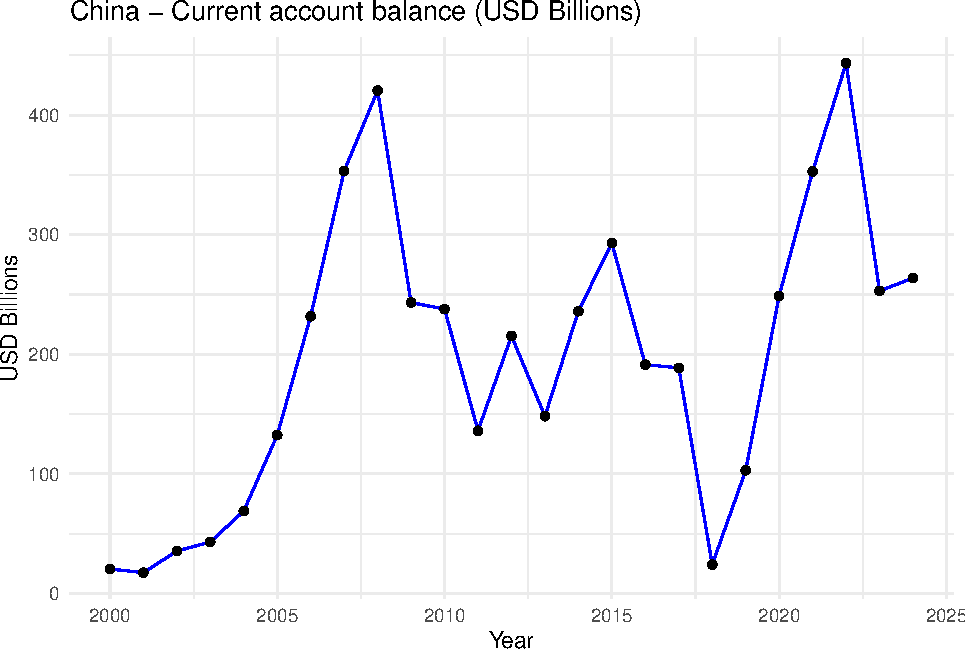
\includegraphics[keepaspectratio]{ProblemSet1_files/figure-latex/unnamed-chunk-2-1.pdf}}
\pandocbounded{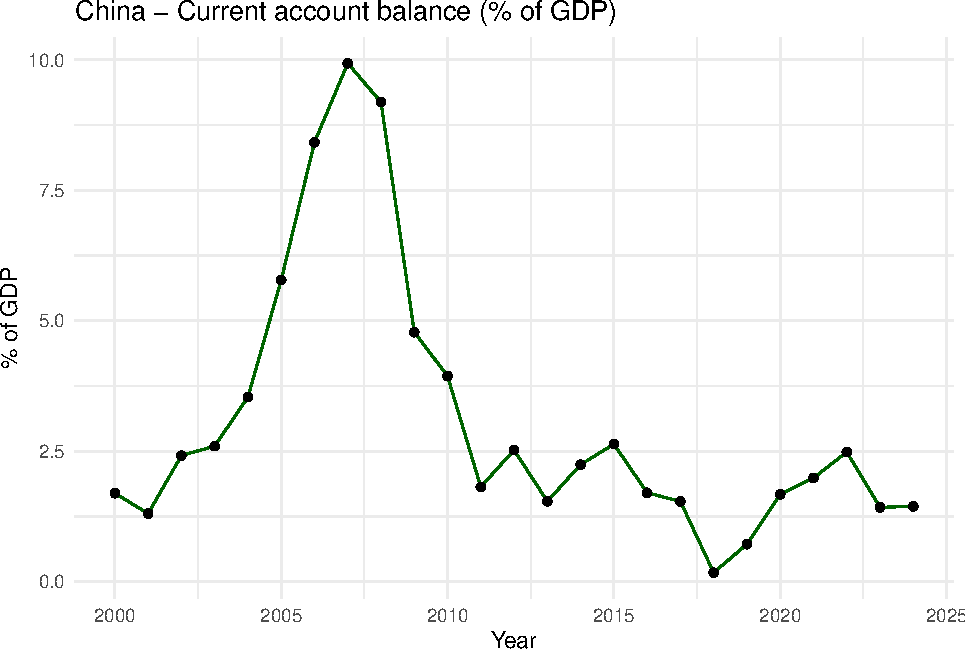
\includegraphics[keepaspectratio]{ProblemSet1_files/figure-latex/unnamed-chunk-2-2.pdf}}

\begin{verbatim}
## Year with largest annual decline in current account surplus: 2023 
## Decline amount: -190.39 billion USD
\end{verbatim}

China experienced the largest drop in current account surplus in 2023,
down by \$190.39 billion.

\subsubsection{For Japan:}\label{for-japan}

Repeat the same analysis as for China.

\begin{verbatim}
## ====== Japan ======
\end{verbatim}

\pandocbounded{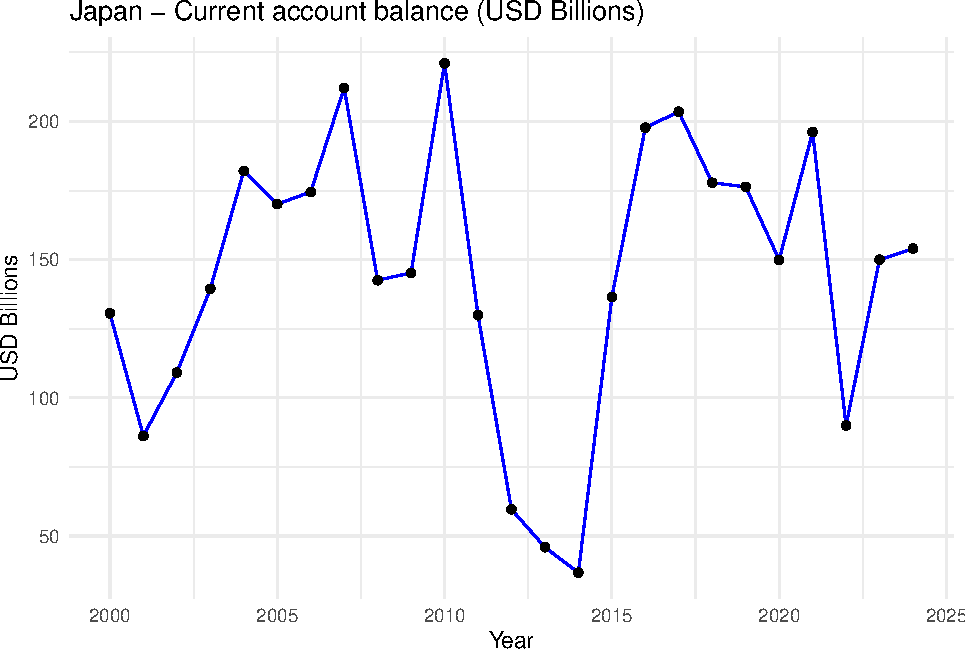
\includegraphics[keepaspectratio]{ProblemSet1_files/figure-latex/unnamed-chunk-3-1.pdf}}
\pandocbounded{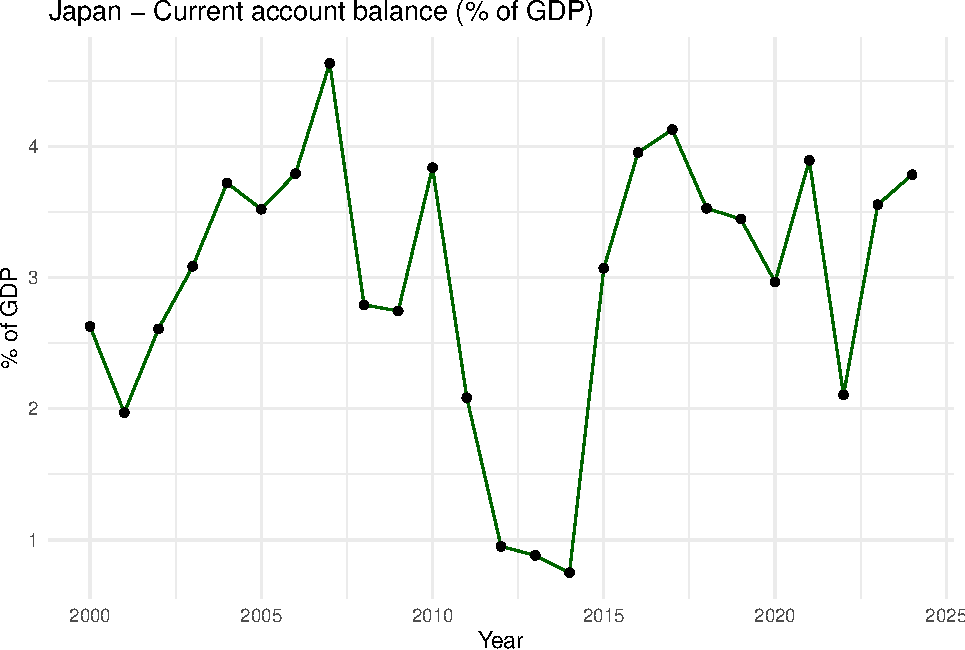
\includegraphics[keepaspectratio]{ProblemSet1_files/figure-latex/unnamed-chunk-3-2.pdf}}

\begin{verbatim}
## Year with largest annual decline in current account surplus: 2022 
## Decline amount: -106.23 billion USD
\end{verbatim}

Japan saw the largest drop in 2022, decreasing by \$106.23 billion.

\subsubsection{For the United States:}\label{for-the-united-states}

Plot both measures and determine the year with the largest annual
increase in current account deficits.

\begin{verbatim}
## ====== United States ======
\end{verbatim}

\pandocbounded{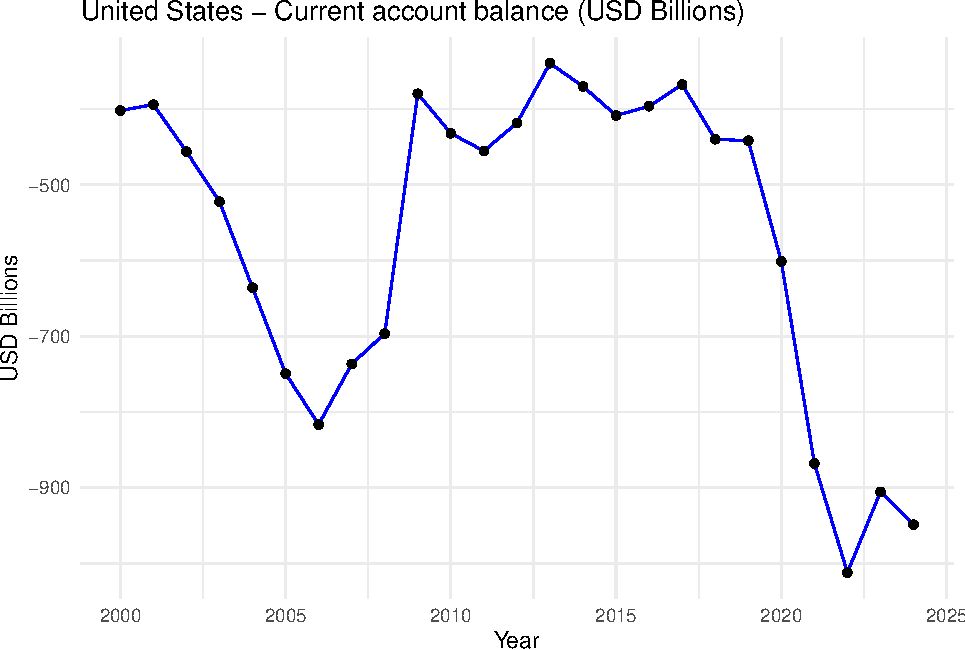
\includegraphics[keepaspectratio]{ProblemSet1_files/figure-latex/unnamed-chunk-4-1.pdf}}
\pandocbounded{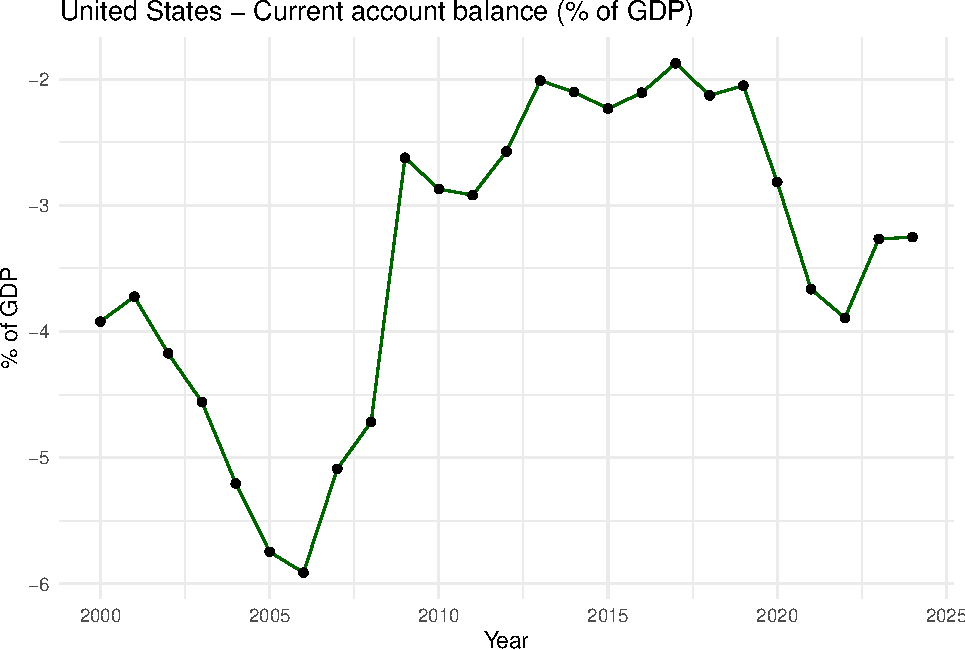
\includegraphics[keepaspectratio]{ProblemSet1_files/figure-latex/unnamed-chunk-4-2.pdf}}

\begin{verbatim}
## Year with largest annual increase in current account deficit: 2021 
## Deficit increase: -266.78 billion USD
\end{verbatim}

The United States had its sharpest increase in deficit in 2021,
worsening by \$266.78 billion.

\subsection{Problem 1.2: Bureau of Economic Analysis (BEA) U.S.
International
Transactions}\label{problem-1.2-bureau-of-economic-analysis-bea-u.s.-international-transactions}

Navigate to Table 1.1. U.S. International Transactions and download the
annual series for Balance on current account (2000--2024) using the
formula Line 1 less Line 9.

\subsubsection{Plot the U.S. current account balance using BEA
data.}\label{plot-the-u.s.-current-account-balance-using-bea-data.}

Compare this graph with the IMF-derived series and highlight
discrepancies (if any).

\begin{verbatim}
## Warning: Using `size` aesthetic for lines was deprecated in ggplot2 3.4.0.
## i Please use `linewidth` instead.
## This warning is displayed once every 8 hours.
## Call `lifecycle::last_lifecycle_warnings()` to see where this warning was
## generated.
\end{verbatim}

\pandocbounded{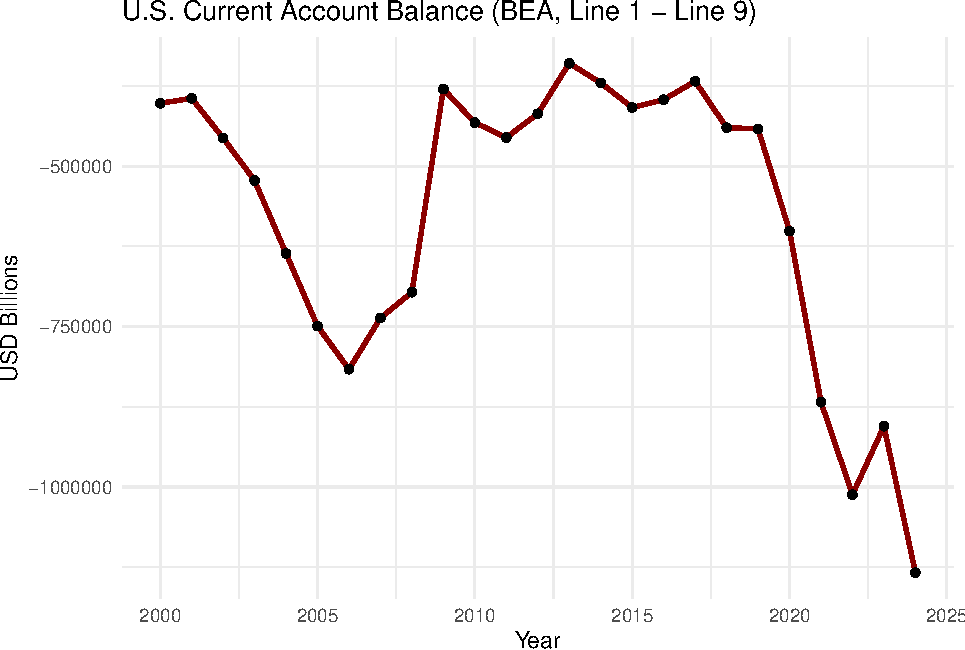
\includegraphics[keepaspectratio]{ProblemSet1_files/figure-latex/unnamed-chunk-6-1.pdf}}
\pandocbounded{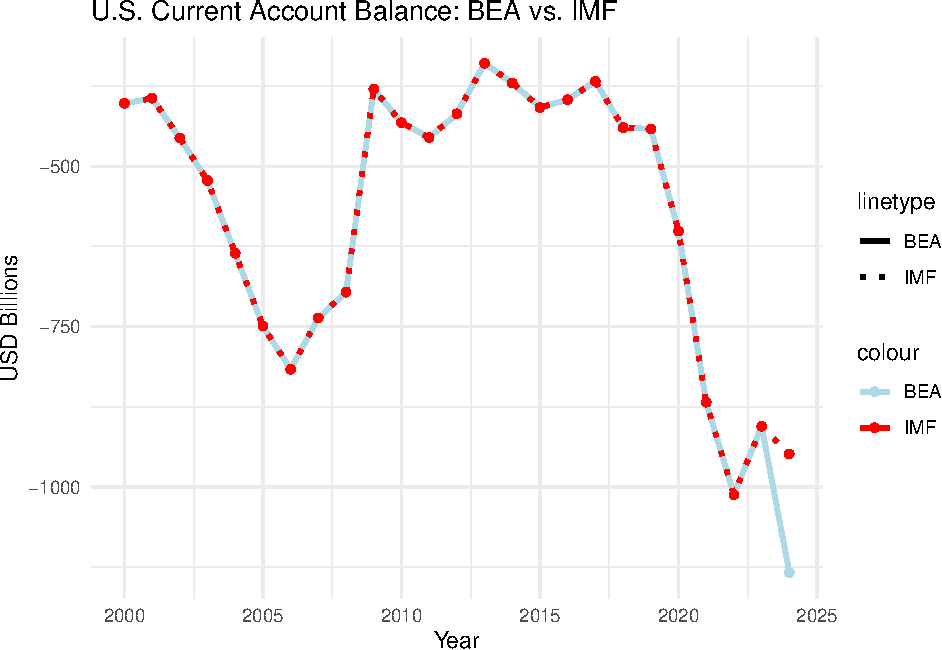
\includegraphics[keepaspectratio]{ProblemSet1_files/figure-latex/unnamed-chunk-6-2.pdf}}

\subsection{Problem 1.3: FRED Download the monthly nominal exchange rate
for Chinese RMB to U.S. Dollar from FRED series DEXCHUS (January 2000 --
January
2025).}\label{problem-1.3-fred-download-the-monthly-nominal-exchange-rate-for-chinese-rmb-to-u.s.-dollar-from-fred-series-dexchus-january-2000-january-2025.}

Obtain the euro to U.S. dollar (EUR/USD) rate for the same period from
FRED.

\subsubsection{Compute the CNY/EUR cross rate using the formula. Plot
the derived cross rate time series and annotate key
trends.}\label{compute-the-cnyeur-cross-rate-using-the-formula.-plot-the-derived-cross-rate-time-series-and-annotate-key-trends.}

Objective: Calculate the monthly \textbf{CNY/EUR cross rate} for the
period \textbf{January 2000 -- January 2025}, using data from the FRED
database: - \textbf{DEXCHUS}: Chinese Yuan per U.S. Dollar (CNY/USD) -
\textbf{DEXUSEU}: U.S. Dollar per Euro (USD/EUR)

Formula:

The CNY/EUR cross rate is computed using the formula:

\[
\text{CNY/EUR} = \frac{\text{CNY/USD}}{\text{USD/EUR}}
\]

This expresses how many Chinese yuan are needed to buy one euro, using
USD as the common denominator.

\begin{verbatim}
## 
## Attaching package: 'lubridate'
\end{verbatim}

\begin{verbatim}
## The following objects are masked from 'package:base':
## 
##     date, intersect, setdiff, union
\end{verbatim}

\begin{verbatim}
## 
## Attaching package: 'zoo'
\end{verbatim}

\begin{verbatim}
## The following objects are masked from 'package:base':
## 
##     as.Date, as.Date.numeric
\end{verbatim}

\pandocbounded{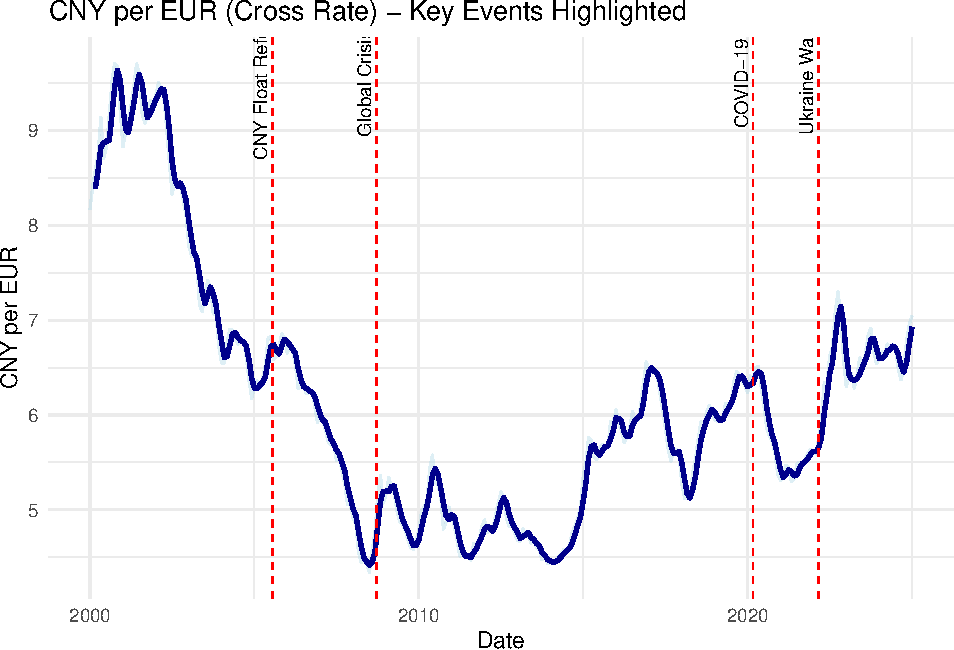
\includegraphics[keepaspectratio]{ProblemSet1_files/figure-latex/unnamed-chunk-7-1.pdf}}

Key Observations: 2000--2005: The CNY/EUR rate was high
(\textasciitilde9.5), reflecting the yuan's peg to the USD and euro
appreciation. 2005-07-21: After the CNY Float Reform, the yuan started a
gradual appreciation. 2008 Global Financial Crisis: Led to euro
appreciation, lowering the CNY/EUR cross rate. 2015--2020: Moderate
volatility and gradual rise in CNY/EUR, signaling RMB weakness.
2022--2023: Spikes due to COVID-19 recovery and Ukraine conflict created
instability.

This analysis illustrates how cross exchange rates can be derived from
bilateral rates and used to monitor relative currency dynamics between
trading blocs (China and Eurozone). Key historical events align closely
with spikes or trends in the CNY/EUR rate, confirming the responsiveness
of currency markets to global shocks and policy shifts.

\section{Problem 2: Exchange Rate Changes and Cross Rate
Calculation}\label{problem-2-exchange-rate-changes-and-cross-rate-calculation}

\subsection{Problem 2(a): Computing Exchange
Rates}\label{problem-2a-computing-exchange-rates}

\textbf{Task:}\\
Compute the U.S. dollar--yen exchange rate \(E_{\$/¥}\) and the U.S.
dollar--Canadian dollar exchange rate \(E_{\$/C\$}\) on January 20,
2016, and January 20, 2015.

\begin{longtable}[]{@{}llrr@{}}
\toprule\noalign{}
Country & Currency & FX\_per\_USD\_2016 & FX\_per\_USD\_2015 \\
\midrule\noalign{}
\endhead
\bottomrule\noalign{}
\endlastfoot
Australia & AUD & 1.459 & 1.223 \\
Canada & CAD & 1.451 & 1.209 \\
Denmark & DKK & 6.844 & 6.430 \\
Eurozone & EUR & 0.917 & 0.865 \\
Hong Kong & HKD & 7.827 & 7.752 \\
India & INR & 68.050 & 61.640 \\
Japan & JPY & 116.380 & 118.480 \\
Mexico & MXN & 18.600 & 14.647 \\
Sweden & SEK & 8.583 & 8.181 \\
UK & GBP & 0.706 & 0.600 \\
USA & USD & 1.000 & 1.000 \\
\end{longtable}

\textbf{Solution:}

\begin{verbatim}
## USD to JPY on Jan 20, 2016: 116.38
\end{verbatim}

\begin{verbatim}
## USD to JPY on Jan 20, 2015: 118.48
\end{verbatim}

\begin{verbatim}
## USD to CAD on Jan 20, 2016: 1.451
\end{verbatim}

\begin{verbatim}
## USD to CAD on Jan 20, 2015: 1.209
\end{verbatim}

\begin{itemize}
\tightlist
\item
  The \textbf{USD/JPY} exchange rate \textbf{decreased} slightly from
  \textbf{118.48 to 116.38}, indicating that the Japanese yen
  \textbf{strengthened} against the U.S. dollar over the year.
\item
  The \textbf{USD/CAD} exchange rate \textbf{increased} from
  \textbf{1.209 to 1.451}, meaning that the Canadian dollar
  \textbf{weakened} against the U.S. dollar during the same period.
\end{itemize}

These changes reflect shifts in relative economic performance, interest
rates, and commodity prices, especially oil (important for Canada).

\subsection{Problem 2(b): Percentage Change in the Value of the U.S.
Dollar}\label{problem-2b-percentage-change-in-the-value-of-the-u.s.-dollar}

We compute the percentage change in the U.S. dollar value relative to
Japanese yen and Canadian dollar using the formula:

\[
\text{Percentage Change} = \left( \frac{E_{t} - E_{t-1}}{E_{t-1}} \right) \times 100
\]

\begin{verbatim}
## USD to JPY % change: -1.77 %
\end{verbatim}

\begin{verbatim}
## USD to CAD % change: 20.02 %
\end{verbatim}

The U.S. dollar depreciated by 1.77\% against the Japanese yen. The U.S.
dollar appreciated by 20.01\% against the Canadian dollar between
January 20, 2015, and January 20, 2016.

\subsection{Problem 2(c): Danish Krone--Canadian Dollar Exchange Rate on
January 20,
2016}\label{problem-2c-danish-kronecanadian-dollar-exchange-rate-on-january-20-2016}

\textbf{Task:}\\
Using the data for January 20, 2016, compute the Danish krone--Canadian
dollar exchange rate \(E_{\text{krone/C\$}}\).

\textbf{Given:}

\begin{itemize}
\tightlist
\item
  Danish krone per U.S. dollar \(E_{\text{krone/\$}} = 6.844\)
\item
  Canadian dollar per U.S. dollar \(E_{\text{CAD/\$}} = 1.451\)
\end{itemize}

We calculate the cross exchange rate using:

\[
E_{\text{krone/C\$}} = \frac{E_{\text{krone/\$}}}{E_{\text{CAD/\$}}}
\]

\begin{verbatim}
## Danish krone per Canadian dollar: 4.7167
\end{verbatim}

On January 20, 2016, 1 Canadian dollar could be exchanged for
approximately 4.7163 Danish kroner.

\section{Problem 3: U.S. Effective Exchange Rate and Bilateral
Changes}\label{problem-3-u.s.-effective-exchange-rate-and-bilateral-changes}

\textbf{Given:} We are provided with trade weights (shares) and exchange
rates for four of the United States' largest trading partners: Canada,
Mexico, China, and Japan. Exchange rates are expressed in \textbf{USD
per unit of foreign currency} for both 2015 and 2016.

\begin{longtable}[]{@{}lrrr@{}}
\toprule\noalign{}
country & share\_trade & USD\_per\_fx\_2015 & USD\_per\_fx\_2016 \\
\midrule\noalign{}
\endhead
\bottomrule\noalign{}
\endlastfoot
Canada & 0.36 & 0.8271 & 0.6892 \\
Mexico & 0.28 & 0.0683 & 0.0538 \\
China & 0.20 & 0.1608 & 0.1522 \\
Japan & 0.16 & 0.0080 & 0.0086 \\
\end{longtable}

\subsection{Problem 3(a) Compute the percentage change in bilateral
exchange rates (USD per
FX):}\label{problem-3a-compute-the-percentage-change-in-bilateral-exchange-rates-usd-per-fx}

The percentage change in each bilateral exchange rate is calculated
using the formula:

\[
\text{Percentage Change} = \left( \frac{E_{2016} - E_{2015}}{E_{2015}} \right) \times 100
\]

\textbf{Results:}

\begin{longtable}[]{@{}lrrrr@{}}
\caption{Bilateral Exchange Rate Changes (USD per FX)}\tabularnewline
\toprule\noalign{}
country & share\_trade & USD\_per\_fx\_2015 & USD\_per\_fx\_2016 &
pct\_change \\
\midrule\noalign{}
\endfirsthead
\toprule\noalign{}
country & share\_trade & USD\_per\_fx\_2015 & USD\_per\_fx\_2016 &
pct\_change \\
\midrule\noalign{}
\endhead
\bottomrule\noalign{}
\endlastfoot
Canada & 0.36 & 0.8271 & 0.6892 & -16.6727 \\
Mexico & 0.28 & 0.0683 & 0.0538 & -21.2299 \\
China & 0.20 & 0.1608 & 0.1522 & -5.3483 \\
Japan & 0.16 & 0.0080 & 0.0086 & 7.5000 \\
\end{longtable}

The U.S. dollar \textbf{depreciated} against the Japanese yen (positive
\% change), but \textbf{appreciated} against the other three currencies
(negative \% change, i.e., fewer dollars per unit of foreign currency).

\subsection{Problem 3(b) Compute the Nominal Effective Exchange Rate
(NEER):}\label{problem-3b-compute-the-nominal-effective-exchange-rate-neer}

We calculate NEER as a \textbf{weighted average} of the bilateral
exchange rates using the trade shares as weights.

\[
\text{NEER}_{2015} = \sum (w_i \cdot E_{2015,i}) = 0.35032 \\
\text{NEER}_{2016} = \sum (w_i \cdot E_{2016,i}) = 0.29499
\]

Then compute the percentage change in NEER:

\[
\text{NEER Change} = \left( \frac{0.29499 - 0.35032}{0.35032} \right) \times 100 \approx -15.79\%
\]

\begin{Shaded}
\begin{Highlighting}[]
\CommentTok{\# ====== (b) NOMINAL EFFECTIVE EXCHANGE RATE (NEER) ======}
\CommentTok{\# Compute NEER for 2015 and 2016}
\NormalTok{neer\_2015 }\OtherTok{\textless{}{-}} \FunctionTok{sum}\NormalTok{(exchange\_rates\_problem\_3}\SpecialCharTok{$}\NormalTok{share\_trade }\SpecialCharTok{*}\NormalTok{ exchange\_rates\_problem\_3}\SpecialCharTok{$}\NormalTok{USD\_per\_fx\_2015)}
\NormalTok{neer\_2016 }\OtherTok{\textless{}{-}} \FunctionTok{sum}\NormalTok{(exchange\_rates\_problem\_3}\SpecialCharTok{$}\NormalTok{share\_trade }\SpecialCharTok{*}\NormalTok{ exchange\_rates\_problem\_3}\SpecialCharTok{$}\NormalTok{USD\_per\_fx\_2016)}

\CommentTok{\# \% Change in NEER}
\NormalTok{neer\_change }\OtherTok{\textless{}{-}}\NormalTok{ (neer\_2016 }\SpecialCharTok{{-}}\NormalTok{ neer\_2015) }\SpecialCharTok{/}\NormalTok{ neer\_2015 }\SpecialCharTok{*} \DecValTok{100}

\FunctionTok{cat}\NormalTok{(}\StringTok{"NEER in 2015:"}\NormalTok{, }\FunctionTok{round}\NormalTok{(neer\_2015, }\DecValTok{5}\NormalTok{), }\StringTok{"}\SpecialCharTok{\textbackslash{}n}\StringTok{"}\NormalTok{)}
\end{Highlighting}
\end{Shaded}

\begin{verbatim}
## NEER in 2015: 0.35032
\end{verbatim}

\begin{Shaded}
\begin{Highlighting}[]
\FunctionTok{cat}\NormalTok{(}\StringTok{"NEER in 2016:"}\NormalTok{, }\FunctionTok{round}\NormalTok{(neer\_2016, }\DecValTok{5}\NormalTok{), }\StringTok{"}\SpecialCharTok{\textbackslash{}n}\StringTok{"}\NormalTok{)}
\end{Highlighting}
\end{Shaded}

\begin{verbatim}
## NEER in 2016: 0.29499
\end{verbatim}

\begin{Shaded}
\begin{Highlighting}[]
\FunctionTok{cat}\NormalTok{(}\StringTok{"Percentage change in NEER:"}\NormalTok{, }\FunctionTok{round}\NormalTok{(neer\_change, }\DecValTok{2}\NormalTok{), }\StringTok{"\%}\SpecialCharTok{\textbackslash{}n}\StringTok{"}\NormalTok{)}
\end{Highlighting}
\end{Shaded}

\begin{verbatim}
## Percentage change in NEER: -15.79 %
\end{verbatim}

\subsection{Problem 3(c) Interpretation and
Comparison:}\label{problem-3c-interpretation-and-comparison}

\begin{itemize}
\tightlist
\item
  The \textbf{nominal effective exchange rate (NEER)} \textbf{fell by
  15.79\%}, meaning that \textbf{the U.S. dollar appreciated} on average
  against this trade-weighted currency basket from 2015 to 2016.
\item
  This appreciation reflects that fewer U.S. dollars were needed per
  unit of foreign currency on average, except for the Japanese yen.
\item
  Compared to the \textbf{Mexican peso}, which saw a \textbf{21.23\%
  depreciation} of the peso relative to the dollar (i.e., the dollar
  strengthened the most against the peso), the effective appreciation of
  the dollar (\textbf{15.79\%}) is slightly less dramatic but still
  significant.
\item
  In summary, the U.S. dollar \textbf{strengthened notably} against most
  major trade partners in this period, with the \textbf{strongest
  bilateral appreciation against the Mexican peso} and a \textbf{modest
  depreciation against the Japanese yen}.
\end{itemize}

\section{Problem 4: Dutch Investor --- Interest Parity and Exchange
Rates}\label{problem-4-dutch-investor-interest-parity-and-exchange-rates}

\textbf{Given:}

\begin{itemize}
\item
  Initial amount: €1,000
\item
  Dutch interest rate: \textbf{5\%}
\item
  British interest rate: \textbf{1\%}
\item
  Spot rate \(E_{\text{spot}}\): \textbf{1.5 euros per pound}
\item
  Forward rate \(E_{\text{forward}}\): \textbf{1.65 euros per pound}
\end{itemize}

\subsection{Problem 4(a) What is the euro-denominated return on Dutch
deposits?}\label{problem-4a-what-is-the-euro-denominated-return-on-dutch-deposits}

This is a \textbf{domestic investment}, so the return is simply the
Dutch interest rate:

\[
\text{Return} = 5\%
\Rightarrow 1000 \times (1 + 0.05) = €1050
\]

\subsection{Problem 4(b) What is the (riskless) euro-denominated return
on British deposits using forward
cover?}\label{problem-4b-what-is-the-riskless-euro-denominated-return-on-british-deposits-using-forward-cover}

Steps: 1. Convert euros to pounds at spot rate:\\
\[
   £ = \frac{1000}{1.5} = £666.67
   \] 2. Earn 1\% interest in Britain:\\
\[
   £666.67 \times 1.01 = £673.33
   \] 3. Convert back to euros at \textbf{forward rate}: \[
   € = £673.33 \times 1.65 = €1110
   \]

\textbf{Return in euros}: \[
\frac{1110 - 1000}{1000} = 11\%
\]

\subsection{Problem 4(c) Is there an arbitrage opportunity? Is this an
equilibrium?}\label{problem-4c-is-there-an-arbitrage-opportunity-is-this-an-equilibrium}

Yes, there \textbf{is an arbitrage opportunity}: - Dutch investment
yields \textbf{5\%} - British investment with forward cover yields
\textbf{11\%}

Since the \textbf{covered return} on British deposits is higher than the
domestic return, a Dutch investor can: - Borrow in euros at 5\%, convert
to pounds, invest in UK at 1\%, and lock in 11\% return using the
forward contract.

This is \textbf{not an equilibrium}, because arbitrage would put upward
pressure on the spot rate (more demand for pounds), and downward
pressure on the forward rate (more forward selling of pounds), until
\textbf{CIP holds}.

\begin{center}\rule{0.5\linewidth}{0.5pt}\end{center}

\subsection{Problem 4(d) What is the equilibrium forward rate according
to
CIP?}\label{problem-4d-what-is-the-equilibrium-forward-rate-according-to-cip}

Using the \textbf{Covered Interest Parity (CIP)} condition:

\[
\frac{1 + i_{\text{€}}}{1 + i_{£}} = \frac{F}{E}
\Rightarrow \frac{1.05}{1.01} = \frac{F}{1.5}
\Rightarrow F = \frac{1.05}{1.01} \times 1.5 \approx 1.56
\]

So, the \textbf{equilibrium forward rate} should be \textbf{€1.56 per
£}.

\subsection{Problem 4(e) Compute the forward premium on the British
pound.}\label{problem-4e-compute-the-forward-premium-on-the-british-pound.}

Forward premium:

\[
\text{Premium} = \frac{F - E}{E} = \frac{1.56 - 1.5}{1.5} = 0.04 = 4\%
\]

\textbf{Answer:} The \textbf{forward premium is +4\%},
i.e.~\textbf{positive}.\\
This is required in equilibrium to offset the lower British interest
rate (1\%) relative to the Dutch rate (5\%), ensuring investors are
indifferent between domestic and foreign deposits when forward cover is
used.

\subsection{Problem 4(f) If UIP holds, what is the expected depreciation
of the
euro?}\label{problem-4f-if-uip-holds-what-is-the-expected-depreciation-of-the-euro}

\textbf{Uncovered Interest Parity (UIP):}

\[
\frac{1 + i_{€}}{1 + i_{£}} = \frac{E^{e}}{E}
\Rightarrow \frac{1.05}{1.01} = \frac{E^{e}}{1.5}
\Rightarrow E^{e} = \frac{1.05}{1.01} \times 1.5 \approx 1.56
\]

So, expected future spot rate is \textbf{€1.56 per £}, implying:

\[
\text{Expected depreciation of euro} = \frac{1.56 - 1.5}{1.5} = 4\%
\]

\subsection{Problem 4(g) Expected euro--pound exchange rate one year
ahead?}\label{problem-4g-expected-europound-exchange-rate-one-year-ahead}

From (f):\\
\[
E^{e}_{1\text{yr}} = €1.56/\text{£}
\]

\textbf{Summary of Answers}

\begin{longtable}[]{@{}ll@{}}
\toprule\noalign{}
Question & Answer \\
\midrule\noalign{}
\endhead
\bottomrule\noalign{}
\endlastfoot
4(a) & 5\% return (€1050) \\
4(b) & 11\% return (€1110) \\
4(c) & Arbitrage exists (not equilibrium) \\
4(d) & Equilibrium forward rate: €1.56/£ \\
4(e) & Forward premium = +4\% (positive) \\
4(f) & Expected depreciation of euro = 4\% \\
4(g) & Expected future rate = €1.56/£ \\
\end{longtable}

\section{Problem 5: Coffee Prices and the Law of One
Price}\label{problem-5-coffee-prices-and-the-law-of-one-price}

\textbf{Given:}

\begin{itemize}
\item
  \textbf{Vietnam price of coffee:} 4,500 VND per pound
\item
  \textbf{Exchange rate:} \(E_{\text{VND/XOF}} = 30\) (30 dong per 1 CFA
  franc)
\item
  \textbf{Côte d'Ivoire price of coffee (observed):} 160 CFA francs per
  pound
\end{itemize}

\subsection{\texorpdfstring{Problem 5(a) What is the price of coffee in
Côte d'Ivoire \textbf{if the law of one price
holds}?}{Problem 5(a) What is the price of coffee in Côte d'Ivoire if the law of one price holds?}}\label{problem-5a-what-is-the-price-of-coffee-in-cuxf4te-divoire-if-the-law-of-one-price-holds}

To convert the Vietnamese price to CFA francs using the exchange rate:

\[
\text{Price in CFA} = \frac{4500 \ \text{VND}}{30 \ \text{VND/XOF}} = 150 \ \text{CFA francs}
\]

\textbf{Answer:}\\
If the \textbf{law of one price} holds, coffee should cost \textbf{150
CFA francs} per pound in Côte d'Ivoire.

\subsection{Problem 5(b) What happens if the actual price in Côte
d'Ivoire is 160 CFA
francs?}\label{problem-5b-what-happens-if-the-actual-price-in-cuxf4te-divoire-is-160-cfa-francs}

\subsubsection{\texorpdfstring{Step 1: Compute the \textbf{relative
price}:}{Step 1: Compute the relative price:}}\label{step-1-compute-the-relative-price}

\[
\text{Relative price (Côte d’Ivoire vs Vietnam)} = \frac{160}{150} = 1.0667
\]

So coffee in Côte d'Ivoire is about \textbf{6.67\% more expensive} than
in Vietnam.

\subsubsection{Step 2: Arbitrage logic:}\label{step-2-arbitrage-logic}

Since coffee is cheaper in Vietnam (after adjusting for exchange rates),
\textbf{traders will:}

\begin{itemize}
\tightlist
\item
  \textbf{Buy coffee in Vietnam} (at 4,500 VND or 150 CFA)
\item
  \textbf{Sell it in Côte d'Ivoire} (at 160 CFA)
\end{itemize}

\subsubsection{Step 3: Market effects:}\label{step-3-market-effects}

\begin{itemize}
\item
  \textbf{In Vietnam:}\\
  Increased demand will \textbf{raise the domestic price} of coffee in
  dong (VND).
\item
  \textbf{In Côte d'Ivoire:}\\
  Increased supply from imports will \textbf{push down the price} of
  coffee in CFA francs.
\end{itemize}

These price movements will continue until the prices equalize across
countries (i.e., the law of one price is restored).

\textbf{Summary of Answers}

\begin{longtable}[]{@{}
  >{\raggedright\arraybackslash}p{(\linewidth - 2\tabcolsep) * \real{0.5556}}
  >{\raggedright\arraybackslash}p{(\linewidth - 2\tabcolsep) * \real{0.4444}}@{}}
\toprule\noalign{}
\begin{minipage}[b]{\linewidth}\raggedright
Question
\end{minipage} & \begin{minipage}[b]{\linewidth}\raggedright
Answer
\end{minipage} \\
\midrule\noalign{}
\endhead
\bottomrule\noalign{}
\endlastfoot
5(a) & Law of one price → 150 CFA francs per pound \\
5(b) & Relative price = 1.0667 (6.67\% higher in Côte d'Ivoire); traders
will buy in Vietnam and sell in Côte d'Ivoire, raising the price in
Vietnam and lowering it in Côte d'Ivoire \\
\end{longtable}

\section{Problem 6: Currency Valuation and Exchange Rate
Expectations}\label{problem-6-currency-valuation-and-exchange-rate-expectations}

We use Purchasing Power Parity (PPP) and Real Exchange Rate (RER)
analysis to assess whether each currency is over- or under-valued
relative to the U.S. dollar and to predict expected real exchange rate
movements.

\begin{Shaded}
\begin{Highlighting}[]
\CommentTok{\# ===== Input Data =====}
\NormalTok{countries }\OtherTok{\textless{}{-}} \FunctionTok{data.frame}\NormalTok{(}
  \AttributeTok{country =} \FunctionTok{c}\NormalTok{(}\StringTok{"Brazil"}\NormalTok{, }\StringTok{"India"}\NormalTok{, }\StringTok{"Mexico"}\NormalTok{, }\StringTok{"South Africa"}\NormalTok{, }\StringTok{"Zimbabwe"}\NormalTok{),}
  \AttributeTok{currency =} \FunctionTok{c}\NormalTok{(}\StringTok{"real"}\NormalTok{, }\StringTok{"rupee"}\NormalTok{, }\StringTok{"peso"}\NormalTok{, }\StringTok{"rand"}\NormalTok{, }\StringTok{"Z$"}\NormalTok{),}
  \AttributeTok{E\_fx\_usd =} \FunctionTok{c}\NormalTok{(}\FloatTok{4.07}\NormalTok{, }\FloatTok{68.51}\NormalTok{, }\FloatTok{18.89}\NormalTok{, }\FloatTok{15.78}\NormalTok{, }\DecValTok{101347}\NormalTok{),}
  \AttributeTok{basket\_local =} \FunctionTok{c}\NormalTok{(}\DecValTok{520}\NormalTok{, }\DecValTok{12000}\NormalTok{, }\DecValTok{1800}\NormalTok{, }\DecValTok{800}\NormalTok{, }\DecValTok{4000000}\NormalTok{)}
\NormalTok{)}

\FunctionTok{kable}\NormalTok{(countries)}
\end{Highlighting}
\end{Shaded}

\begin{longtable}[]{@{}llrr@{}}
\toprule\noalign{}
country & currency & E\_fx\_usd & basket\_local \\
\midrule\noalign{}
\endhead
\bottomrule\noalign{}
\endlastfoot
Brazil & real & 4.07 & 520 \\
India & rupee & 68.51 & 12000 \\
Mexico & peso & 18.89 & 1800 \\
South Africa & rand & 15.78 & 800 \\
Zimbabwe & Z\$ & 101347.00 & 4000000 \\
\end{longtable}

\textbf{Formula used:}

\begin{itemize}
\tightlist
\item
  Real Exchange Rate (RER):\\
  \[
  \text{RER} = \frac{E_{\text{FX}/\$} \times P_{US}}{P_{\text{local}}}
  \]
\item
  PPP holds when RER ≈ 1
\end{itemize}

\textbf{U.S. price of the basket:} \$190

\textbf{Results:}

\begin{longtable}[]{@{}
  >{\raggedright\arraybackslash}p{(\linewidth - 14\tabcolsep) * \real{0.1103}}
  >{\raggedright\arraybackslash}p{(\linewidth - 14\tabcolsep) * \real{0.1241}}
  >{\raggedright\arraybackslash}p{(\linewidth - 14\tabcolsep) * \real{0.1655}}
  >{\raggedright\arraybackslash}p{(\linewidth - 14\tabcolsep) * \real{0.1448}}
  >{\raggedright\arraybackslash}p{(\linewidth - 14\tabcolsep) * \real{0.0483}}
  >{\raggedright\arraybackslash}p{(\linewidth - 14\tabcolsep) * \real{0.0897}}
  >{\raggedright\arraybackslash}p{(\linewidth - 14\tabcolsep) * \real{0.1517}}
  >{\raggedright\arraybackslash}p{(\linewidth - 14\tabcolsep) * \real{0.1655}}@{}}
\toprule\noalign{}
\begin{minipage}[b]{\linewidth}\raggedright
Country
\end{minipage} & \begin{minipage}[b]{\linewidth}\raggedright
FX Rate (per \$)
\end{minipage} & \begin{minipage}[b]{\linewidth}\raggedright
Basket Price (Local)
\end{minipage} & \begin{minipage}[b]{\linewidth}\raggedright
Basket Price (USD)
\end{minipage} & \begin{minipage}[b]{\linewidth}\raggedright
RER
\end{minipage} & \begin{minipage}[b]{\linewidth}\raggedright
PPP Holds?
\end{minipage} & \begin{minipage}[b]{\linewidth}\raggedright
Currency Valuation
\end{minipage} & \begin{minipage}[b]{\linewidth}\raggedright
Expected RER Movement
\end{minipage} \\
\midrule\noalign{}
\endhead
\bottomrule\noalign{}
\endlastfoot
Brazil & 4.07 & 520 & 127.76 & 1.487 & No & Under-valued &
Appreciation \\
India & 68.51 & 12,000 & 175.16 & 1.085 & No & Under-valued &
Appreciation \\
Mexico & 18.89 & 1,800 & 95.29 & 1.994 & No & Under-valued &
Appreciation \\
South Africa & 15.78 & 800 & 50.70 & 3.748 & No & Under-valued &
Appreciation \\
Zimbabwe & 101,347.00 & 4,000,000 & 39.47 & 4.814 & No & Under-valued &
Appreciation \\
\end{longtable}

\begin{itemize}
\item
  \textbf{Brazil:} The real exchange rate is 1.487, meaning goods are
  cheaper in Brazil than in the U.S. in real terms. The Brazilian real
  is \textbf{under-valued}, and we should expect \textbf{real
  appreciation} in the long run.
\item
  \textbf{India:} With RER = 1.085, the rupee is slightly under-valued.
  PPP does not hold, so \textbf{real appreciation} is expected.
\item
  \textbf{Mexico:} A much lower basket cost in USD terms (95.29) implies
  significant under-valuation of the peso. RER = 1.994 suggests goods
  are much cheaper in Mexico, pointing to \textbf{expected real
  appreciation}.
\item
  \textbf{South Africa:} RER = 3.748 is quite high, indicating that the
  rand is substantially \textbf{under-valued}. Real appreciation is
  expected.
\item
  \textbf{Zimbabwe:} With RER = 4.814, the Zimbabwean dollar is heavily
  \textbf{under-valued}, suggesting significant room for \textbf{real
  appreciation} relative to the USD if markets move toward equilibrium.
\end{itemize}

For all countries listed, PPP does \textbf{not} hold, and their
currencies appear to be \textbf{under-valued} relative to the USD.
Therefore, in the long run, we expect their real exchange rates to
\textbf{appreciate}, aligning with the theory of purchasing power
parity.

\section{Problem 7: Real Exchange Rate and Inflation
Expectations}\label{problem-7-real-exchange-rate-and-inflation-expectations}

\textbf{Given:}

\begin{itemize}
\item
  Current nominal exchange rate: \textbf{\$1.5/£}
\item
  U.S. basket price: \textbf{\$100}
\item
  Same basket in U.K.: \textbf{£120}
\item
  U.S. inflation (π\_US): \textbf{2\%}
\item
  U.K. inflation (π\_UK): \textbf{3\%}
\item
  Speed of convergence to PPP: \textbf{15\% per year}
\end{itemize}

\subsection{Problem 7(a) What is the expected U.S. minus U.K. inflation
differential?}\label{problem-7a-what-is-the-expected-u.s.-minus-u.k.-inflation-differential}

\[
\pi_{\text{US}} - \pi_{\text{UK}} = 2\% - 3\% = -1\%
\]

\textbf{Answer:} \textbf{--1\%} (i.e., U.K. inflation is higher by 1\%).

\subsection{\texorpdfstring{Problem 7(b) What is the current U.S. real
exchange rate \(q_{\text{US/UK}}\) with the
U.K.?}{Problem 7(b) What is the current U.S. real exchange rate q\_\{\textbackslash text\{US/UK\}\} with the U.K.?}}\label{problem-7b-what-is-the-current-u.s.-real-exchange-rate-q_textusuk-with-the-u.k.}

Real exchange rate formula: \[
q = \frac{E \cdot P_{UK}}{P_{US}} = \frac{1.5 \cdot 120}{100} = 1.8
\]

\textbf{Answer:} The current real exchange rate is \textbf{1.8}.

\subsection{Problem 7(c) How much is the dollar
overvalued/undervalued?}\label{problem-7c-how-much-is-the-dollar-overvaluedundervalued}

If \(q > 1\), the dollar is \textbf{overvalued}.

\[
\% \text{overvaluation} = (q - 1) \times 100 = (1.8 - 1) \times 100 = 80\%
\]

\textbf{Answer:} The dollar is \textbf{overvalued by 80\%} relative to
the pound.

\subsection{Problem 7(d) What will be the real exchange rate in one
year?}\label{problem-7d-what-will-be-the-real-exchange-rate-in-one-year}

Real exchange rate converges toward 1 (PPP level) by 15\% per year:

\[
q_{t+1} = q_t - \lambda (q_t - 1) = 1.8 - 0.15(1.8 - 1) = 1.8 - 0.15(0.8) = 1.68
\]

\textbf{Answer:} Real exchange rate in one year is expected to be
\textbf{1.68}

\subsection{Problem 7(e) What is the expected rate of real depreciation
for the
U.S.?}\label{problem-7e-what-is-the-expected-rate-of-real-depreciation-for-the-u.s.}

\[
\text{Rate of real depreciation} = \frac{q_{t+1} - q_t}{q_t} = \frac{1.68 - 1.8}{1.8} = -0.0667 = -6.67\%
\]

\textbf{Answer:} \textbf{--6.67\%} (i.e., the U.S. dollar is expected to
\textbf{appreciate in real terms})

\subsection{\texorpdfstring{Problem 7(f) What is the expected rate of
\textbf{nominal depreciation} for the
U.S.?}{Problem 7(f) What is the expected rate of nominal depreciation for the U.S.?}}\label{problem-7f-what-is-the-expected-rate-of-nominal-depreciation-for-the-u.s.}

\[
\text{Nominal depreciation} = \text{real depreciation} + \text{inflation differential} \\
= (-6.67\%) + (-1\%) = -7.67\%
\]

\textbf{Answer:} \textbf{--7.67\%} (i.e., the nominal value of the
dollar is expected to \textbf{appreciate})

\subsection{\texorpdfstring{Problem 7(g) What do you predict will be the
\textbf{dollar price of one pound} in one
year?}{Problem 7(g) What do you predict will be the dollar price of one pound in one year?}}\label{problem-7g-what-do-you-predict-will-be-the-dollar-price-of-one-pound-in-one-year}

Current nominal exchange rate: \(E = 1.5\)\\
Nominal depreciation rate = --7.67\%\\
\[
E_{t+1} = E_t \cdot (1 + \text{depreciation}) = 1.5 \cdot (1 - 0.0767) \approx 1.385
\]

\textbf{Answer:} The expected exchange rate in one year is
\textbf{\$1.385/£}

\textbf{Summary of Answers}

\begin{longtable}[]{@{}ll@{}}
\toprule\noalign{}
Question & Answer \\
\midrule\noalign{}
\endhead
\bottomrule\noalign{}
\endlastfoot
7(a) & --1\% inflation differential \\
7(b) & Real exchange rate = 1.8 \\
7(c) & Dollar is 80\% overvalued \\
7(d) & Expected real exchange rate = 1.68 \\
7(e) & Real depreciation rate = --6.67\% \\
7(f) & Nominal depreciation rate = --7.67\% \\
7(g) & Expected exchange rate in one year = \textbf{\$1.385/£} \\
\end{longtable}

\section{Problem 8: Simple Monetary Model -- Korea and Japan
(1996)}\label{problem-8-simple-monetary-model-korea-and-japan-1996}

\textbf{Given:}

\begin{itemize}
\tightlist
\item
  \textbf{Japan}:

  \begin{itemize}
  \tightlist
  \item
    Output growth \(g_J = 1\%\)
  \item
    Money growth \(\mu_J = 2\%\)
  \end{itemize}
\item
  \textbf{South Korea}:

  \begin{itemize}
  \tightlist
  \item
    Output growth \(g_K = 6\%\)
  \item
    Money growth \(\mu_K = 15\%\)
  \end{itemize}
\end{itemize}

According to the \textbf{Simple Monetary Model} with constant velocity:

\[
\pi = \mu - g
\]

Where: - \(\pi\): inflation - \(\mu\): money growth rate - \(g\): output
growth rate

\subsection{Problem 8(a) What is the inflation rate in South Korea? In
Japan?}\label{problem-8a-what-is-the-inflation-rate-in-south-korea-in-japan}

Using \(\pi = \mu - g\):

\begin{itemize}
\item
  \textbf{Korea:}\\
  \[
  \pi_K = 15\% - 6\% = 9\%
  \]
\item
  \textbf{Japan:}\\
  \[
  \pi_J = 2\% - 1\% = 1\%
  \]
\end{itemize}

\textbf{Answer:}\\
- South Korea inflation = \textbf{9\%}\\
- Japan inflation = \textbf{1\%}

\subsection{Problem 8(b) Expected depreciation rate of the Korean won
relative to the Japanese
yen?}\label{problem-8b-expected-depreciation-rate-of-the-korean-won-relative-to-the-japanese-yen}

According to \textbf{Purchasing Power Parity (PPP)}:

\[
\text{Depreciation of won} = \pi_K - \pi_J = 9\% - 1\% = 8\%
\]

\textbf{Answer:}\\
Expected depreciation of the won = \textbf{8\%}

\subsection{Problem 8(c) New Korean inflation rate if money growth drops
to
12\%?}\label{problem-8c-new-korean-inflation-rate-if-money-growth-drops-to-12}

\[
\pi_K^{\text{new}} = 12\% - 6\% = 6\%
\]

\textbf{Answer:}\\
New Korean inflation rate = \textbf{6\%}

\subsection{Problem 8(d) Time series diagram
interpretation}\label{problem-8d-time-series-diagram-interpretation}

If the Bank of Korea \textbf{increases} money growth (e.g., from 12\% to
15\% again), the following happens over time:

\begin{longtable}[]{@{}
  >{\raggedright\arraybackslash}p{(\linewidth - 2\tabcolsep) * \real{0.4706}}
  >{\raggedright\arraybackslash}p{(\linewidth - 2\tabcolsep) * \real{0.5294}}@{}}
\toprule\noalign{}
\begin{minipage}[b]{\linewidth}\raggedright
Variable
\end{minipage} & \begin{minipage}[b]{\linewidth}\raggedright
Effect over time
\end{minipage} \\
\midrule\noalign{}
\endhead
\bottomrule\noalign{}
\endlastfoot
\(M_K\) (Money supply) & Increases more rapidly \\
\(i_K\) (Nominal interest rate) & Rises \\
\(P_K\) (Price level) & Increases (faster inflation) \\
Real money balances \(M_K/P_K\) & Eventually return to previous level
(short-run dip) \\
Exchange rate \(E_{\text{won}/¥}\) & Depreciates over time \\
\end{longtable}

\textbf{Diagram axes (for all plots):}\\
- \textbf{x-axis}: Time\\
- \textbf{y-axis}: Variable level

Each plot would show a shift in trend or kink in the trajectory of each
variable starting at the policy change point (e.g., t₀).

\subsection{Problem 8(e) What money growth rate is needed to maintain a
fixed exchange rate
(peg)?}\label{problem-8e-what-money-growth-rate-is-needed-to-maintain-a-fixed-exchange-rate-peg}

For a \textbf{fixed exchange rate}, monetary model implies:

\[
\pi_K = \pi_J \Rightarrow \mu_K - g_K = \mu_J - g_J
\]

Solve for \(\mu_K\):

\[
\mu_K = \mu_J - g_J + g_K = 2\% - 1\% + 6\% = 7\%
\]

\textbf{Answer:}\\
Bank of Korea must adopt a money growth rate of \textbf{7\%} to keep the
won/yen exchange rate fixed.

\subsection{Problem 8(f) What money growth rates would cause the Korean
won to
appreciate?}\label{problem-8f-what-money-growth-rates-would-cause-the-korean-won-to-appreciate}

For the \textbf{won to appreciate}, we need:

\[
\pi_K < \pi_J \Rightarrow \mu_K - g_K < \mu_J - g_J
\Rightarrow \mu_K < \mu_J - g_J + g_K = 7\%
\]

\textbf{Answer:}\\
To appreciate the won, Korea's money growth rate must be \textbf{less
than 7\%}

That is: \[
\boxed{0\% < \mu_K < 7\%}
\]

\textbf{Summary of Answers}

\begin{longtable}[]{@{}
  >{\raggedright\arraybackslash}p{(\linewidth - 2\tabcolsep) * \real{0.5556}}
  >{\raggedright\arraybackslash}p{(\linewidth - 2\tabcolsep) * \real{0.4444}}@{}}
\toprule\noalign{}
\begin{minipage}[b]{\linewidth}\raggedright
Question
\end{minipage} & \begin{minipage}[b]{\linewidth}\raggedright
Answer
\end{minipage} \\
\midrule\noalign{}
\endhead
\bottomrule\noalign{}
\endlastfoot
(a) & Korea: 9\%, Japan: 1\% inflation \\
(b) & Won expected to depreciate by 8\% \\
(c) & New Korea inflation = 6\% \\
(d) & Increase in money growth → ↑ \(M_K\), ↑ \(i_K\), ↑ \(P_K\), ↓ real
money balances, ↑ exchange rate \(E_{\text{won}/¥}\) \\
(e) & To fix exchange rate, \(\mu_K = 7\%\) \\
(f) & For appreciation, \(0\% < \mu_K < 7\%\) \\
\end{longtable}

\section{Problem 9: General Monetary Model -- Korea and
Japan}\label{problem-9-general-monetary-model-korea-and-japan}

We now use the \textbf{general monetary model}, where \textbf{money
demand depends inversely on the nominal interest rate}. All assumptions
from \textbf{Problem 8} still hold, with the additional information:

\begin{itemize}
\tightlist
\item
  Interest rate in Japan: \(i_{¥} = 3\%\)
\item
  Initial Korean money growth rate: \(\mu_K = 15\%\), output growth =
  6\%
\item
  Inflation in Korea (from Problem 8): \(\pi_K = 9\%\)
\item
  Inflation in Japan: \(\pi_J = 1\%\)
\end{itemize}

\subsection{Problem 9(a) What is the interest rate paid on South Korean
deposits?}\label{problem-9a-what-is-the-interest-rate-paid-on-south-korean-deposits}

We use the \textbf{Fisher equation}:

\[
i = r + \pi
\]

Assuming \textbf{real interest rates are equal} (initially), and using
\(r = i_J - \pi_J = 3\% - 1\% = 2\%\), then:

\[
i_K = r + \pi_K = 2\% + 9\% = 11\%
\]

\textbf{Answer:} The Korean nominal interest rate is \textbf{11\%}

\subsection{Problem 9(b) Show that real interest rates are equal in
Japan and South
Korea}\label{problem-9b-show-that-real-interest-rates-are-equal-in-japan-and-south-korea}

Using:

\[
r = i - \pi
\]

\begin{itemize}
\tightlist
\item
  Japan: \(r_J = 3\% - 1\% = 2\%\)
\item
  Korea: \(r_K = 11\% - 9\% = 2\%\)
\end{itemize}

The \textbf{real interest rates are equal} across countries, consistent
with capital mobility and uncovered interest parity.

\subsection{Problem 9(c) What happens to the Korean interest rate if
money growth falls to
12\%?}\label{problem-9c-what-happens-to-the-korean-interest-rate-if-money-growth-falls-to-12}

If money growth drops from 15\% to 12\%, and inflation drops one-for-one
(output growth unchanged at 6\%):

\[
\pi_K^{\text{new}} = 12\% - 6\% = 6\%
\]

Real interest rate remains \textbf{unchanged} at 2\%, so:

\[
i_K^{\text{new}} = r + \pi_K^{\text{new}} = 2\% + 6\% = 8\%
\]

\textbf{Answer:}

Nominal interest rate in Korea \textbf{falls from 11\% to 8\%}

\subsection{Problem 9(d) Time series diagrams: Effect of lower money
growth}\label{problem-9d-time-series-diagrams-effect-of-lower-money-growth}

If the Bank of Korea reduces money growth from 15\% → 12\%, we expect
the following over time:

\begin{longtable}[]{@{}
  >{\raggedright\arraybackslash}p{(\linewidth - 2\tabcolsep) * \real{0.4000}}
  >{\raggedright\arraybackslash}p{(\linewidth - 2\tabcolsep) * \real{0.6000}}@{}}
\toprule\noalign{}
\begin{minipage}[b]{\linewidth}\raggedright
Variable
\end{minipage} & \begin{minipage}[b]{\linewidth}\raggedright
Time Path Description
\end{minipage} \\
\midrule\noalign{}
\endhead
\bottomrule\noalign{}
\endlastfoot
\(M_K\) (Money supply) & Growth slows down \\
\(i_K\) (Interest rate) & Falls from 11\% → 8\% \\
\(P_K\) (Price level) & Inflation slows (lower slope) \\
\(M_K / P_K\) (Real money balances) & Rises (lower inflation + lower
interest rate) increases money demand \\
\(E_{\text{won}/¥}\) & Depreciation slows; possibly temporary
appreciation \\
\end{longtable}

\textbf{Graph behavior:} - All variables plotted with \textbf{time on
x-axis} - Inflection or kink occurs at the policy change point (e.g.,
time t₀)

\textbf{Key Point:}\\
Lower money growth leads to \textbf{disinflation}, lower interest rates,
and \textbf{higher real money balances}. Nominal depreciation of the won
slows (or reverses), possibly leading to \textbf{short-run
appreciation}.

\textbf{Summary of Answers}

\begin{longtable}[]{@{}
  >{\raggedright\arraybackslash}p{(\linewidth - 2\tabcolsep) * \real{0.5556}}
  >{\raggedright\arraybackslash}p{(\linewidth - 2\tabcolsep) * \real{0.4444}}@{}}
\toprule\noalign{}
\begin{minipage}[b]{\linewidth}\raggedright
Question
\end{minipage} & \begin{minipage}[b]{\linewidth}\raggedright
Answer
\end{minipage} \\
\midrule\noalign{}
\endhead
\bottomrule\noalign{}
\endlastfoot
(a) & \(i_K = 11\%\) \\
(b) & \(r_J = r_K = 2\%\) \\
(c) & New \(i_K = 8\%\) after disinflation \\
(d) & ↓ \(M_K\) growth, ↓ \(i_K\), ↓ inflation, ↑ real balances, slower
depreciation (or appreciation) \\
\end{longtable}

\section{Problem 10: U.S. Money Supply and Exchange Rate
Dynamics}\label{problem-10-u.s.-money-supply-and-exchange-rate-dynamics}

We analyze the effects of a \textbf{temporary increase in the U.S. money
supply} on the \textbf{money market} and \textbf{foreign exchange
market} between the \textbf{U.S. dollar (\$)} and the \textbf{British
pound (£)}. The exchange rate is defined as \(E_{\$/£}\): the number of
dollars per pound.

We use time series diagrams to track the impact over time and mark the
initial equilibrium as point \textbf{A}, the \textbf{short-run
adjustment} as point \textbf{B}, and the \textbf{long-run outcome} as
point \textbf{C}.

\pandocbounded{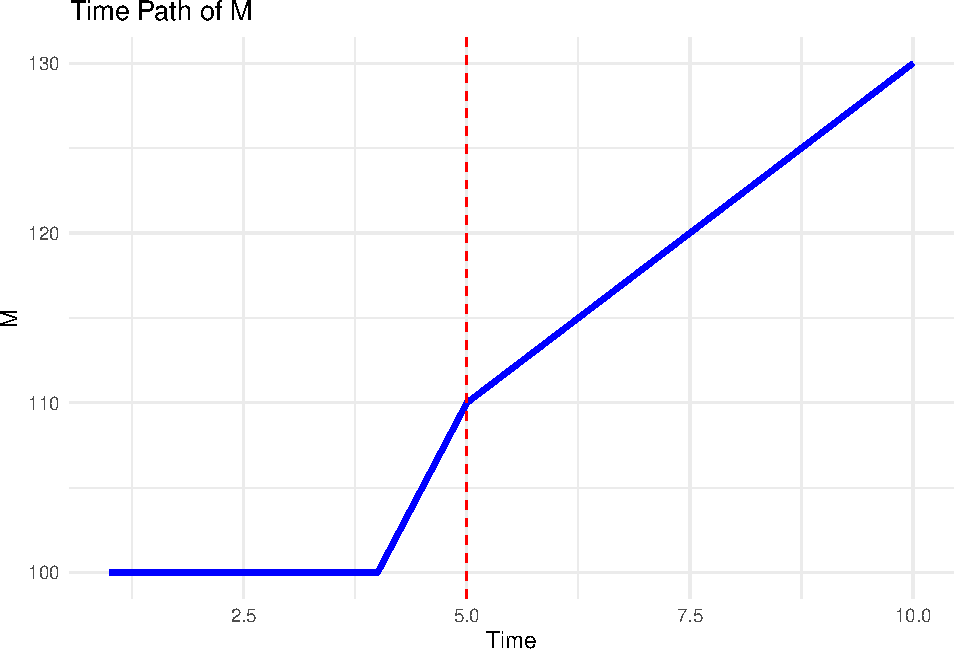
\includegraphics[keepaspectratio]{ProblemSet1_files/figure-latex/unnamed-chunk-17-1.pdf}}
\pandocbounded{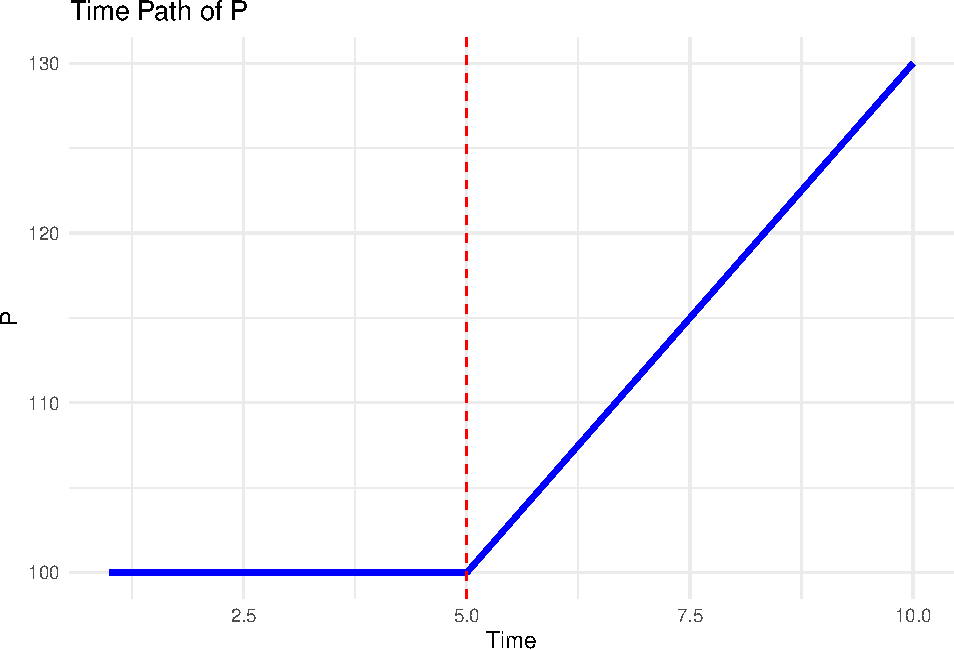
\includegraphics[keepaspectratio]{ProblemSet1_files/figure-latex/unnamed-chunk-17-2.pdf}}
\pandocbounded{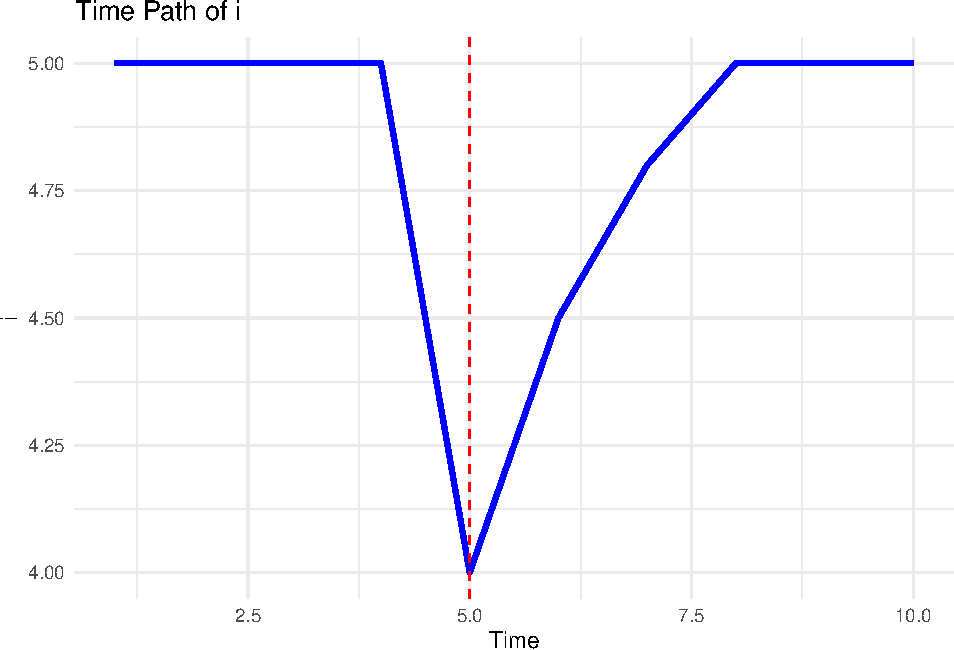
\includegraphics[keepaspectratio]{ProblemSet1_files/figure-latex/unnamed-chunk-17-3.pdf}}
\pandocbounded{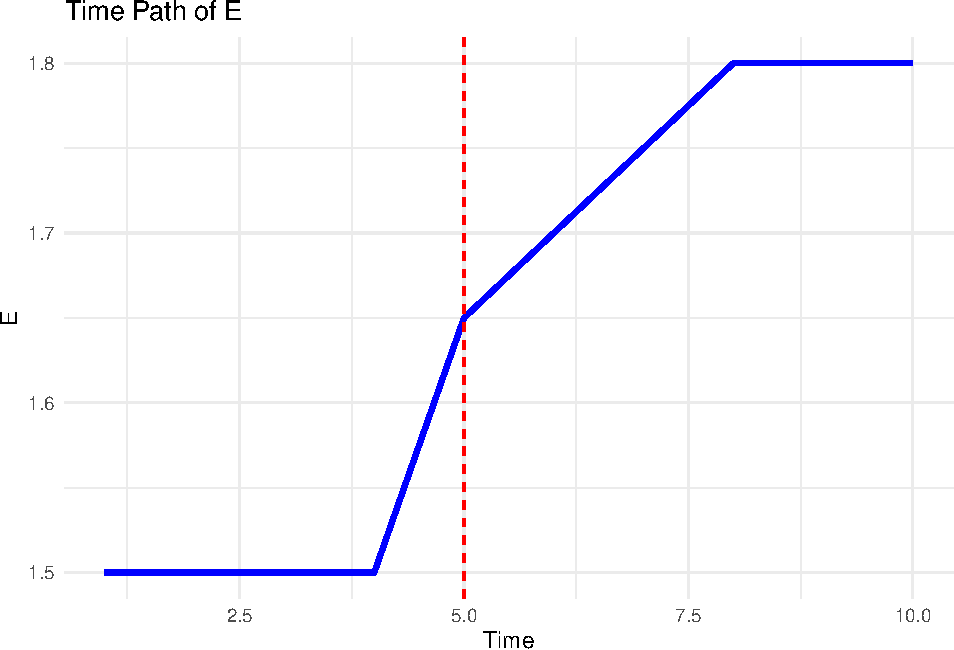
\includegraphics[keepaspectratio]{ProblemSet1_files/figure-latex/unnamed-chunk-17-4.pdf}}
\pandocbounded{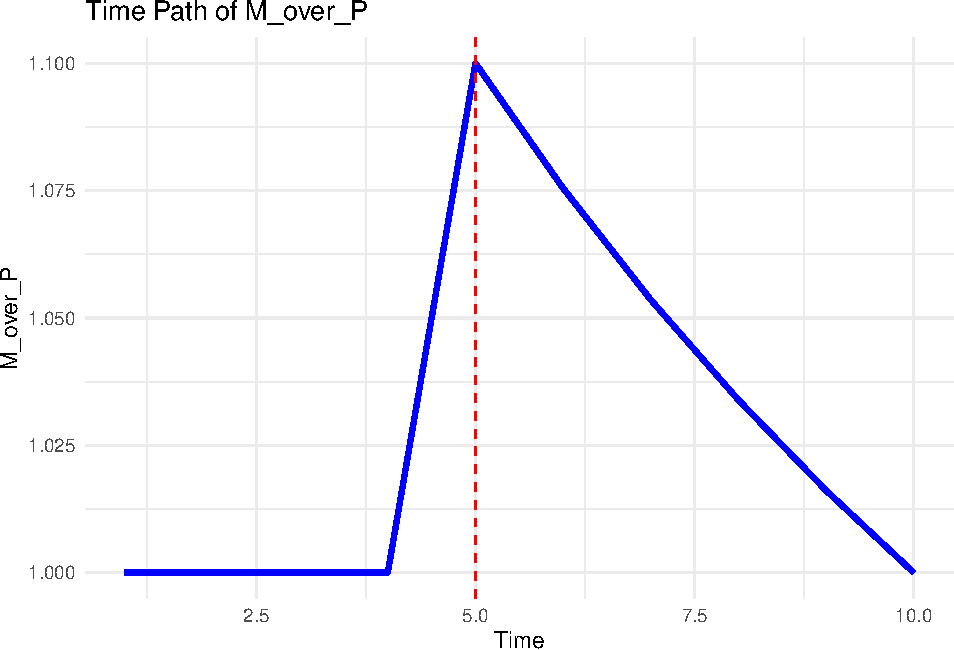
\includegraphics[keepaspectratio]{ProblemSet1_files/figure-latex/unnamed-chunk-17-5.pdf}}

\textbf{Diagram Summary:} My time series plots illustrate:

\begin{itemize}
\item
  \textbf{M (Money Supply):} increases at time t = 5
\item
  \textbf{i (Interest Rate):} falls temporarily, then recovers
\item
  \textbf{P (Price Level):} rises after the lag
\item
  \textbf{M/P (Real Money Balances):} initially increases, then falls
  back
\item
  \textbf{E (\$/£):} dollar depreciates in both short run and long run
\end{itemize}

\subsection{Problem 10(a) Diagram Interpretation: Temporary Increase in
U.S. Money
Supply}\label{problem-10a-diagram-interpretation-temporary-increase-in-u.s.-money-supply}

\begin{itemize}
\item
  \textbf{Money Market:}\\
  The increase in \(M\) shifts the money supply rightward. With sticky
  prices in the short run, the real money supply \(M/P\) rises, leading
  to a \textbf{drop in U.S. interest rates}. This is reflected as a
  movement from point A to point B.
\item
  \textbf{FX Market:}\\
  The lower U.S. interest rate makes U.S. assets less attractive.
  Capital outflows occur, causing the dollar to \textbf{depreciate} and
  \(E_{\$/£}\) to \textbf{increase}.\\
  In the long run, prices \(P\) adjust upward, reducing real money
  balances and returning interest rates to their initial level. The
  exchange rate depreciates \textbf{further}, reaching point C.
\item
  \textbf{Real Money Balances \(M/P\):}\\
  Initially rise due to unchanged prices and higher \(M\), then fall as
  prices catch up, returning to the original level.
\end{itemize}

\subsection{Problem 10(b) Short-run Effects (Point B compared to
A):}\label{problem-10b-short-run-effects-point-b-compared-to-a}

\begin{longtable}[]{@{}
  >{\raggedright\arraybackslash}p{(\linewidth - 4\tabcolsep) * \real{0.5088}}
  >{\raggedright\arraybackslash}p{(\linewidth - 4\tabcolsep) * \real{0.2632}}
  >{\raggedright\arraybackslash}p{(\linewidth - 4\tabcolsep) * \real{0.2281}}@{}}
\toprule\noalign{}
\begin{minipage}[b]{\linewidth}\raggedright
Variable
\end{minipage} & \begin{minipage}[b]{\linewidth}\raggedright
Change
\end{minipage} & \begin{minipage}[b]{\linewidth}\raggedright
Explanation
\end{minipage} \\
\midrule\noalign{}
\endhead
\bottomrule\noalign{}
\endlastfoot
U.S. interest rate \(i_{\$}\) & \textbf{↓} & Liquidity increases,
interest rate falls \\
British interest rate \(i_{£}\) & \textbf{No change} & No policy change
in the U.K. \\
Exchange rate \(E_{\$/£}\) & \textbf{↑} (depreciation) & Dollar weakens
relative to the pound \\
Expected exchange rate \(E^e_{\$/£}\) & \textbf{No change} & Short-run
expectations unchanged \\
U.S. price level \(P\) & \textbf{No change} & Prices are sticky in the
short run \\
\end{longtable}

\subsection{Problem 10(c) Long-run Effects (Point C compared to
A):}\label{problem-10c-long-run-effects-point-c-compared-to-a}

\begin{longtable}[]{@{}
  >{\raggedright\arraybackslash}p{(\linewidth - 4\tabcolsep) * \real{0.5088}}
  >{\raggedright\arraybackslash}p{(\linewidth - 4\tabcolsep) * \real{0.2632}}
  >{\raggedright\arraybackslash}p{(\linewidth - 4\tabcolsep) * \real{0.2281}}@{}}
\toprule\noalign{}
\begin{minipage}[b]{\linewidth}\raggedright
Variable
\end{minipage} & \begin{minipage}[b]{\linewidth}\raggedright
Change
\end{minipage} & \begin{minipage}[b]{\linewidth}\raggedright
Explanation
\end{minipage} \\
\midrule\noalign{}
\endhead
\bottomrule\noalign{}
\endlastfoot
U.S. interest rate \(i_{\$}\) & \textbf{No change} & Returns to initial
level as \(M/P\) normalizes \\
British interest rate \(i_{£}\) & \textbf{No change} & Still no change
in U.K. policy \\
Exchange rate \(E_{\$/£}\) & \textbf{↑} & Dollar permanently depreciates
due to higher \(M\) and \(P\) \\
Expected exchange rate \(E^e_{\$/£}\) & \textbf{↑} & Increases to match
new expected future rate \\
U.S. price level \(P\) & \textbf{↑} & Adjusts upward due to excess
demand for goods \\
\end{longtable}

A \textbf{temporary increase in the U.S. money supply} results in:

\begin{itemize}
\tightlist
\item
  \textbf{Short-run:} lower interest rates and dollar depreciation
  (movement to point B)
\item
  \textbf{Long-run:} higher price level, real money balances return to
  normal, and permanent dollar depreciation (point C)
\end{itemize}

This behavior is consistent with standard monetary models and PPP
adjustment over time.

\section{Problem 11: Impact of a Permanent Decrease in India's Money
Supply}\label{problem-11-impact-of-a-permanent-decrease-in-indias-money-supply}

We analyze the effects of a \textbf{permanent decrease in India's
nominal money supply (M\_IN)} on:

\begin{itemize}
\tightlist
\item
  The \textbf{money market} (interest rates, real balances)
\item
  The \textbf{foreign exchange market} (exchange rate
  \(E_{\text{Rs}/\$}\))
\item
  The \textbf{price level} in India \(P_{\text{IN}}\)
\end{itemize}

The exchange rate is defined as \textbf{rupees per dollar (Rs/\$)} ---
i.e., \textbf{an increase in \(E_{\text{Rs}/\$}\)} means \textbf{rupee
depreciation}, and a decrease means \textbf{rupee appreciation}.

\subsection{Problem 11(a) Diagram Analysis: Money and FX
Markets}\label{problem-11a-diagram-analysis-money-and-fx-markets}

\textbf{Money Market:}

\begin{itemize}
\tightlist
\item
  A \textbf{permanent decrease} in the Indian money supply shifts the
  nominal money supply curve \textbf{left}.
\item
  In the \textbf{short run}, prices are sticky ⇒ real money balances
  \(M/P\) fall ⇒ interest rate in India \textbf{rises}.
\item
  Higher interest rates make Indian assets more attractive.
\end{itemize}

\textbf{FX Market:}

\begin{itemize}
\tightlist
\item
  Higher Indian interest rates lead to \textbf{capital inflows}.
\item
  The rupee \textbf{appreciates sharply} in the short run (point B).
\item
  In the \textbf{long run}, the domestic price level \(P\) decreases in
  proportion to the fall in \(M\).
\item
  Real balances \(M/P\) normalize, and interest rates return to original
  levels (point C).
\item
  The exchange rate settles at a \textbf{permanently appreciated level}.
\end{itemize}

\pandocbounded{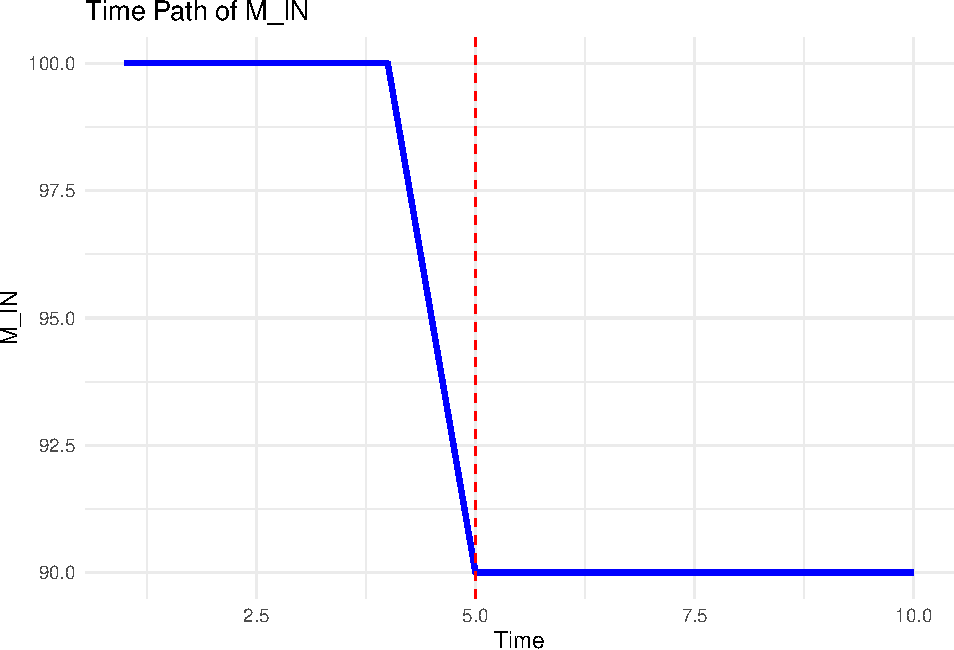
\includegraphics[keepaspectratio]{ProblemSet1_files/figure-latex/unnamed-chunk-18-1.pdf}}
\pandocbounded{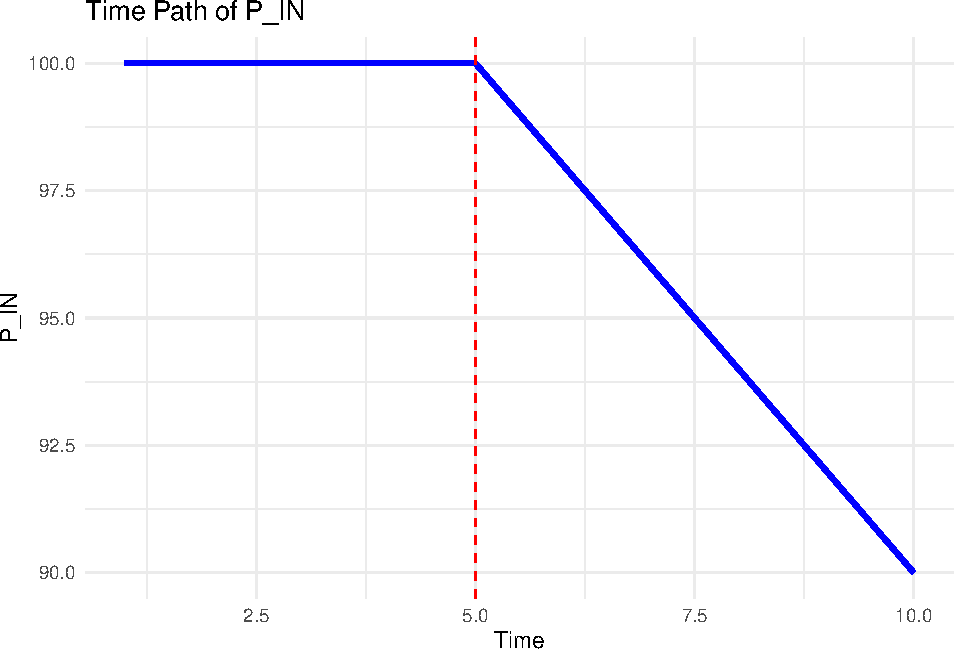
\includegraphics[keepaspectratio]{ProblemSet1_files/figure-latex/unnamed-chunk-18-2.pdf}}
\pandocbounded{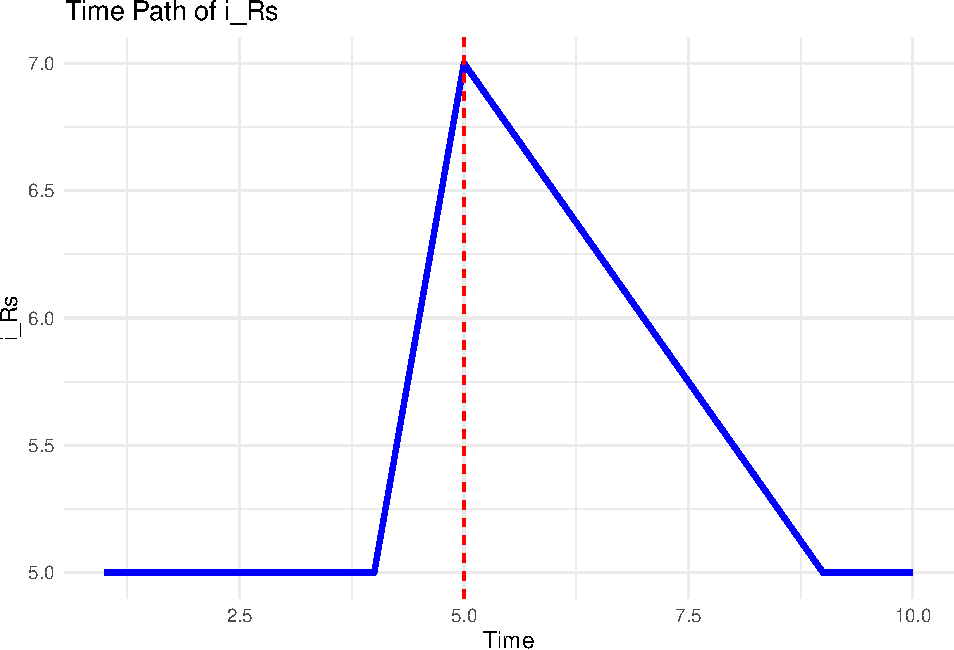
\includegraphics[keepaspectratio]{ProblemSet1_files/figure-latex/unnamed-chunk-18-3.pdf}}
\pandocbounded{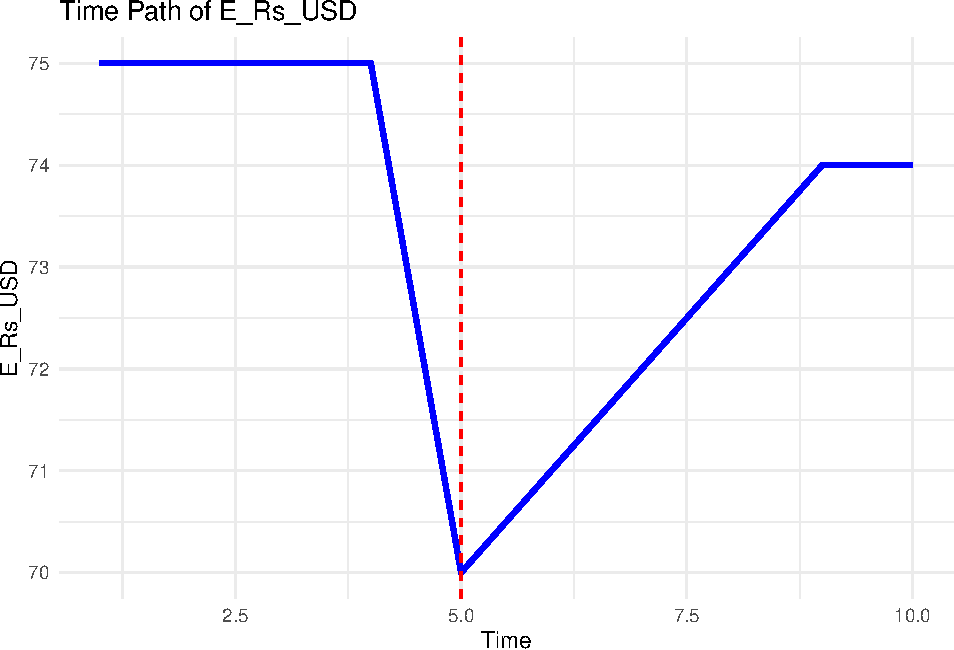
\includegraphics[keepaspectratio]{ProblemSet1_files/figure-latex/unnamed-chunk-18-4.pdf}}
\pandocbounded{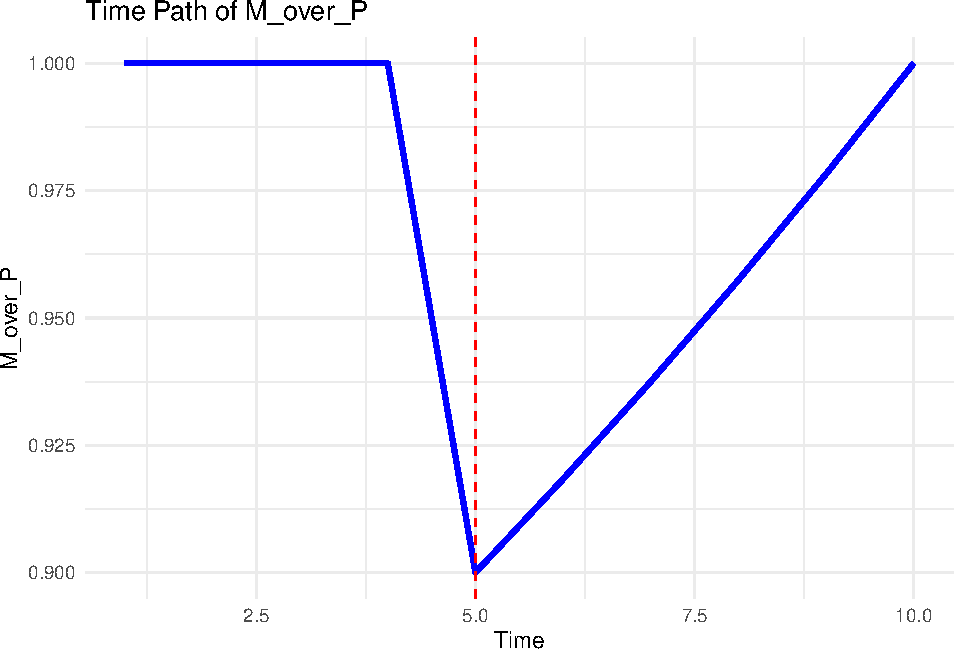
\includegraphics[keepaspectratio]{ProblemSet1_files/figure-latex/unnamed-chunk-18-5.pdf}}

\subsection{Problem 11(b) Time Path of Variables
(India)}\label{problem-11b-time-path-of-variables-india}

On a chart with \textbf{time on the x-axis}, we expect the following:

\begin{longtable}[]{@{}
  >{\raggedright\arraybackslash}p{(\linewidth - 2\tabcolsep) * \real{0.4286}}
  >{\raggedright\arraybackslash}p{(\linewidth - 2\tabcolsep) * \real{0.5714}}@{}}
\toprule\noalign{}
\begin{minipage}[b]{\linewidth}\raggedright
Variable
\end{minipage} & \begin{minipage}[b]{\linewidth}\raggedright
Time Path Description
\end{minipage} \\
\midrule\noalign{}
\endhead
\bottomrule\noalign{}
\endlastfoot
\(M_{IN}\) & Drops permanently at t = A \\
\(P_{IN}\) & Sticky in short run, slowly declines \\
\(M/P\) & Falls sharply (short run), then gradually rises as \(P\)
adjusts \\
\(i_{Rs}\) & Jumps up (short run), then returns to initial level \\
\(E_{\text{Rs}/\$}\) & Overshoots downward (strong rupee appreciation),
then stabilizes at a lower level \\
\end{longtable}

\subsection{Problem 11(c) Short-Run Effects (Point B vs Point
A)}\label{problem-11c-short-run-effects-point-b-vs-point-a}

\begin{longtable}[]{@{}
  >{\raggedright\arraybackslash}p{(\linewidth - 4\tabcolsep) * \real{0.4681}}
  >{\raggedright\arraybackslash}p{(\linewidth - 4\tabcolsep) * \real{0.2553}}
  >{\raggedright\arraybackslash}p{(\linewidth - 4\tabcolsep) * \real{0.2766}}@{}}
\toprule\noalign{}
\begin{minipage}[b]{\linewidth}\raggedright
Variable
\end{minipage} & \begin{minipage}[b]{\linewidth}\raggedright
Change
\end{minipage} & \begin{minipage}[b]{\linewidth}\raggedright
Explanation
\end{minipage} \\
\midrule\noalign{}
\endhead
\bottomrule\noalign{}
\endlastfoot
\(i_{Rs}\) & \textbf{↑} & Money supply ↓ ⇒ liquidity tightens ⇒ rates
↑ \\
\(E_{\text{Rs}/\$}\) & \textbf{↓} (rupee appreciates) & Higher interest
rate attracts capital \\
\(E^e_{\text{Rs}/\$}\) & \textbf{No change} & Expected future exchange
rate unchanged in short run \\
\(P_{IN}\) & \textbf{No change} & Prices are sticky in the short run \\
\end{longtable}

\subsection{Problem 11(d) Long-Run Effects (Point C vs Point
A)}\label{problem-11d-long-run-effects-point-c-vs-point-a}

\begin{longtable}[]{@{}
  >{\raggedright\arraybackslash}p{(\linewidth - 4\tabcolsep) * \real{0.4314}}
  >{\raggedright\arraybackslash}p{(\linewidth - 4\tabcolsep) * \real{0.3137}}
  >{\raggedright\arraybackslash}p{(\linewidth - 4\tabcolsep) * \real{0.2549}}@{}}
\toprule\noalign{}
\begin{minipage}[b]{\linewidth}\raggedright
Variable
\end{minipage} & \begin{minipage}[b]{\linewidth}\raggedright
Change
\end{minipage} & \begin{minipage}[b]{\linewidth}\raggedright
Explanation
\end{minipage} \\
\midrule\noalign{}
\endhead
\bottomrule\noalign{}
\endlastfoot
\(i_{Rs}\) & \textbf{No change} & Real balances return to equilibrium,
so interest rate normalizes \\
\(E_{\text{Rs}/\$}\) & \textbf{↓} (permanent rupee appreciation) & Price
level adjusts downward ⇒ stronger real currency \\
\(E^e_{\text{Rs}/\$}\) & \textbf{↓} & Long-run expectations adjust to
new exchange rate \\
\(P_{IN}\) & \textbf{↓} & Falls to match reduced money supply \\
\end{longtable}

\subsection{Problem 11(e) Overshooting: Theory \&
Practice}\label{problem-11e-overshooting-theory-practice}

\textbf{In theory:}

\begin{itemize}
\tightlist
\item
  According to \textbf{Dornbusch's overshooting model}, exchange rates
  respond \textbf{more than proportionally} in the short run to monetary
  shocks due to sticky prices and fast-moving asset markets.
\item
  In this case, the \textbf{rupee appreciates more than it does in the
  long run}, and then \textbf{partially reverses} as prices adjust
  downward.
\item
  This is the \textbf{overshooting} effect: short-run exchange rate
  movement \textbf{exceeds} its new long-run level.
\end{itemize}

\textbf{In practice:}

\begin{itemize}
\tightlist
\item
  Financial markets react immediately to news (e.g., central bank
  policy).
\item
  Goods markets adjust slowly ⇒ real variables overshoot and stabilize.
\item
  Overshooting can lead to volatility and speculative flows before
  convergence.
\end{itemize}

\textbf{Conclusion:}

A \textbf{permanent decrease in India's money supply} leads to:

\begin{itemize}
\tightlist
\item
  \textbf{Short-run appreciation} of the rupee and \textbf{rise in
  interest rates}.
\item
  \textbf{Long-run price level decline}, return of real balances and
  interest rates to original levels.
\item
  \textbf{Permanent nominal appreciation} of the rupee.
\item
  \textbf{Overshooting}: exchange rate appreciates \emph{more} in the
  short run than in the long run.
\end{itemize}

\section{Problem 12: Is Overshooting Consistent with Purchasing Power
Parity?}\label{problem-12-is-overshooting-consistent-with-purchasing-power-parity}

\textbf{Question:} Is \textbf{overshooting} --- both in theory and in
practice --- consistent with \textbf{Purchasing Power Parity (PPP)}?\\
What are the roles of PPP in the short run vs.~long run, and how do
assumptions in the asset approach affect this?\\
How does overshooting help explain empirical exchange rate behavior?

\textbf{Overshooting and PPP: Are They Consistent?}

\textbf{Yes --- overshooting is consistent with PPP, but only in the
long run.}

\begin{itemize}
\item
  \textbf{PPP} (Purchasing Power Parity) posits that in the \textbf{long
  run}, exchange rates adjust to equalize the prices of identical goods
  across countries:

  \[
  E = \frac{P_{\text{home}}}{P_{\text{foreign}}}
  \]
\item
  \textbf{Overshooting}, as developed in \textbf{Dornbusch's model},
  refers to the phenomenon where the exchange rate responds \textbf{more
  than proportionally} in the \textbf{short run} to a monetary shock due
  to:

  \begin{itemize}
  \tightlist
  \item
    \textbf{Sticky prices} (goods markets adjust slowly)
  \item
    \textbf{Flexible financial markets} (interest rates and capital
    flows adjust quickly)
  \end{itemize}
\end{itemize}

Thus, overshooting describes \textbf{how the exchange rate moves in the
short run} before converging to the level consistent with PPP.

\pandocbounded{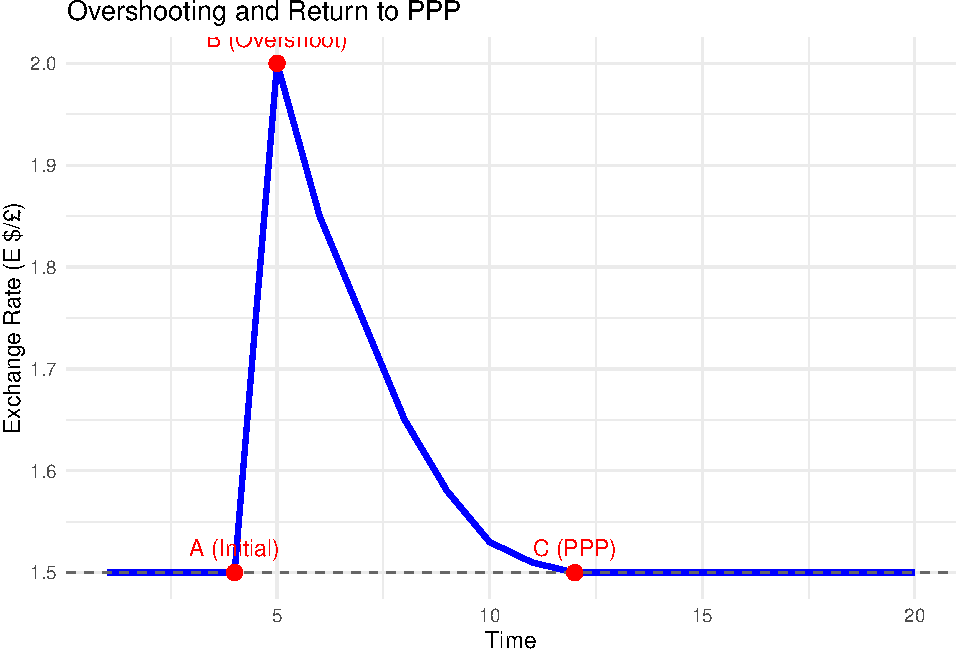
\includegraphics[keepaspectratio]{ProblemSet1_files/figure-latex/unnamed-chunk-19-1.pdf}}

\textbf{PP in the Short Run vs.~Long Run}

\begin{longtable}[]{@{}
  >{\raggedright\arraybackslash}p{(\linewidth - 4\tabcolsep) * \real{0.1566}}
  >{\raggedright\arraybackslash}p{(\linewidth - 4\tabcolsep) * \real{0.4096}}
  >{\raggedright\arraybackslash}p{(\linewidth - 4\tabcolsep) * \real{0.4337}}@{}}
\toprule\noalign{}
\begin{minipage}[b]{\linewidth}\raggedright
Term
\end{minipage} & \begin{minipage}[b]{\linewidth}\raggedright
Short Run
\end{minipage} & \begin{minipage}[b]{\linewidth}\raggedright
Long Run
\end{minipage} \\
\midrule\noalign{}
\endhead
\bottomrule\noalign{}
\endlastfoot
\textbf{PPP validity} & Often \textbf{violated} due to sticky prices,
transaction costs, and non-tradables & More likely to hold as prices
adjust \\
\textbf{Usefulness} & Not a good predictor of short-run exchange rate &
Useful anchor for long-term expectations \\
\textbf{Role} & Not binding; relative prices don't adjust instantly &
Acts as long-run equilibrium condition \\
\end{longtable}

\textbf{Asset Market Approach: Assumptions}

\begin{itemize}
\tightlist
\item
  In the \textbf{short run}, the asset approach assumes:

  \begin{itemize}
  \tightlist
  \item
    \textbf{Capital mobility}
  \item
    Investors reallocate portfolios based on \textbf{interest
    differentials and expectations}
  \item
    Prices are \textbf{sticky}
  \end{itemize}
\item
  In the \textbf{long run}:

  \begin{itemize}
  \tightlist
  \item
    Prices are flexible
  \item
    Real money balances return to normal
  \item
    PPP is restored
  \end{itemize}
\end{itemize}

Overshooting emerges \textbf{because} these asset markets respond
quickly while goods prices do not.

\textbf{How Overshooting Explains Exchange Rate Behavior}

\textbf{Empirical facts:} - Exchange rates are \textbf{highly volatile}
in the short run - They often \textbf{overreact} to news (e.g., monetary
policy) - Long-run exchange rate paths tend to \textbf{revert toward PPP
levels}

\textbf{Overshooting explains this by showing:} - Immediate overreaction
to monetary shocks due to rapid capital flows - Slow correction over
time as price levels catch up - Why real exchange rates can deviate from
1 for long periods

\textbf{Conclusion}

\begin{itemize}
\tightlist
\item
  \textbf{Overshooting is consistent with PPP in the long run}, though
  PPP does \textbf{not hold in the short run}.
\item
  It helps reconcile \textbf{short-term volatility} in exchange rates
  with \textbf{long-run equilibrium theories}.
\item
  PPP remains a \textbf{long-run anchor}, while overshooting explains
  \textbf{short-run deviations} driven by interest rates and
  expectations.
\end{itemize}

\section{Problem 13: Effect of Reduced U.S. Real Money
Demand}\label{problem-13-effect-of-reduced-u.s.-real-money-demand}

We examine the effects of a \textbf{decline in real money demand in the
U.S.}, using \textbf{money market} and \textbf{foreign exchange (FX)}
diagrams. The exchange rate is expressed as \textbf{dollars per euro
\(E_{\$/€}\)} --- an increase in \(E\) implies a \textbf{depreciation of
the U.S. dollar}.

\pandocbounded{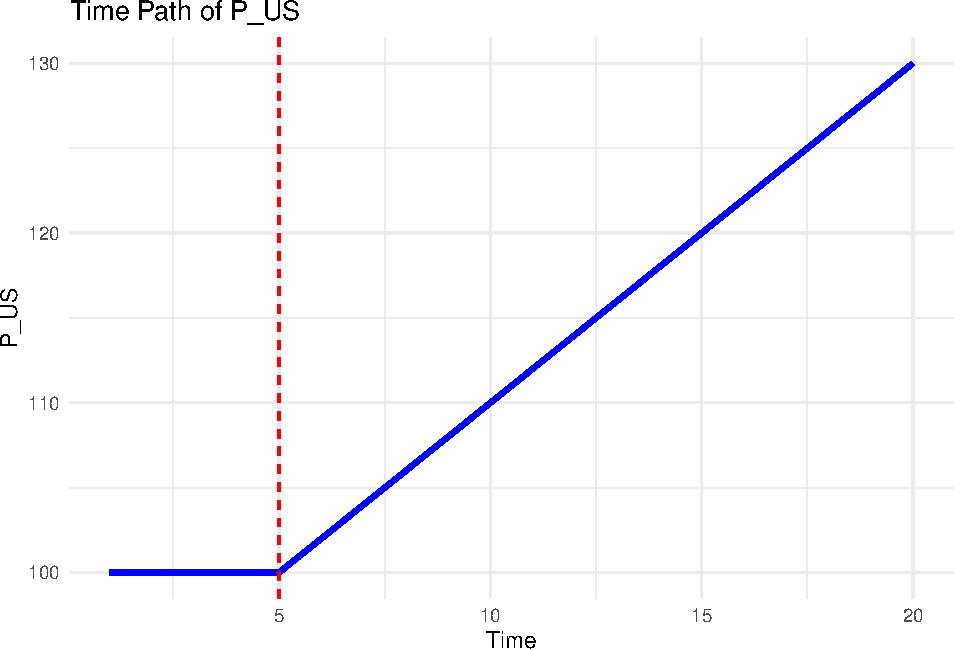
\includegraphics[keepaspectratio]{ProblemSet1_files/figure-latex/unnamed-chunk-20-1.pdf}}
\pandocbounded{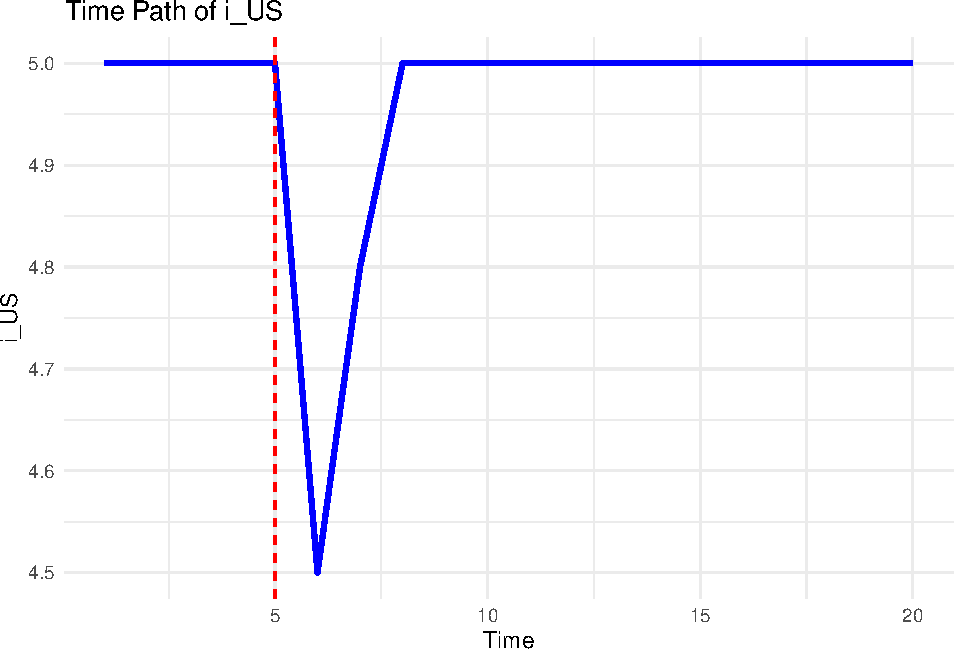
\includegraphics[keepaspectratio]{ProblemSet1_files/figure-latex/unnamed-chunk-20-2.pdf}}
\pandocbounded{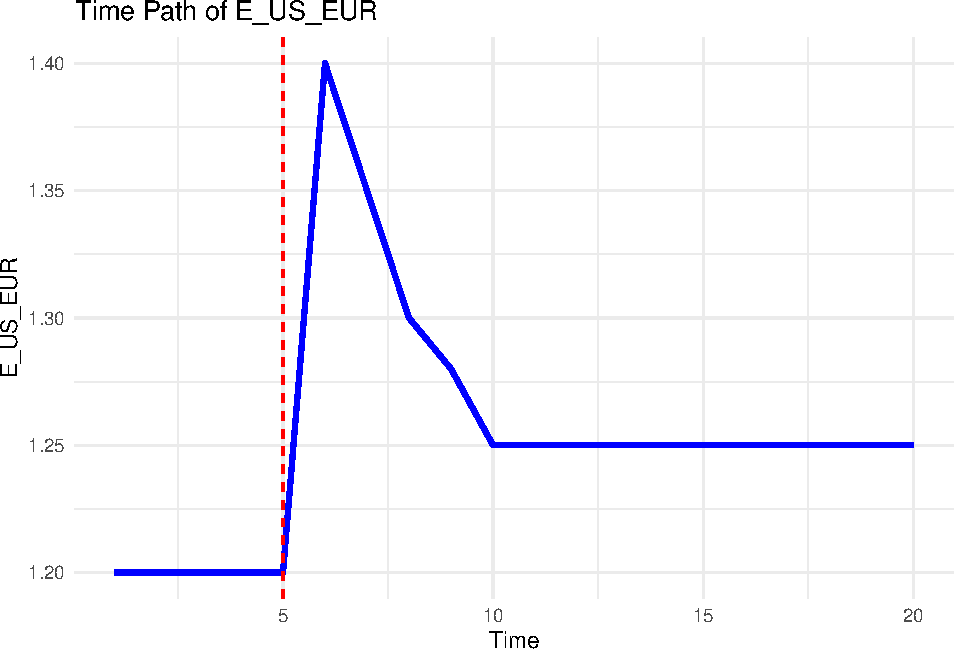
\includegraphics[keepaspectratio]{ProblemSet1_files/figure-latex/unnamed-chunk-20-3.pdf}}
\pandocbounded{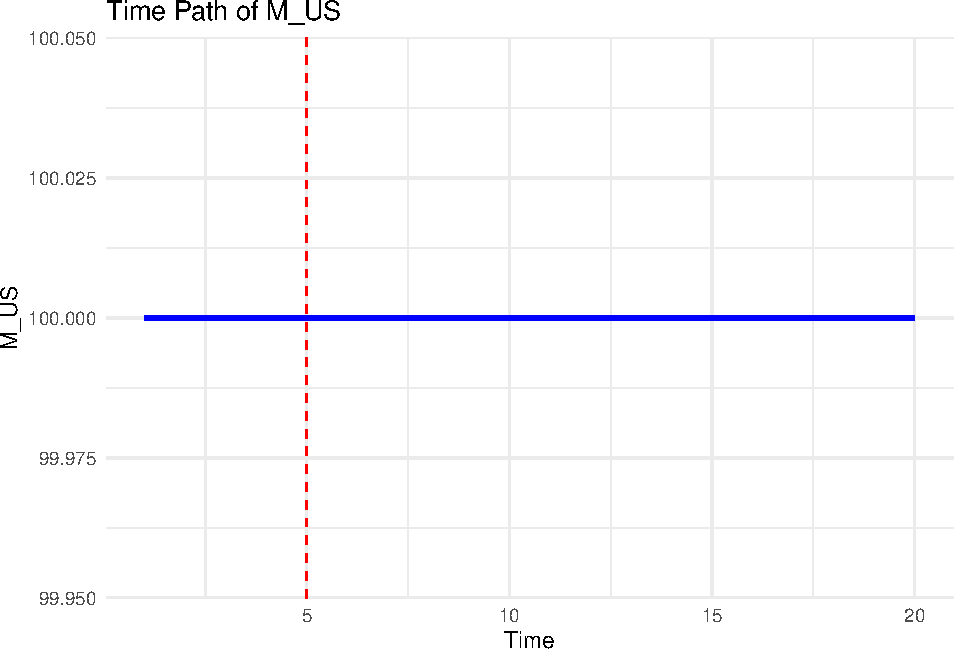
\includegraphics[keepaspectratio]{ProblemSet1_files/figure-latex/unnamed-chunk-20-4.pdf}}
\pandocbounded{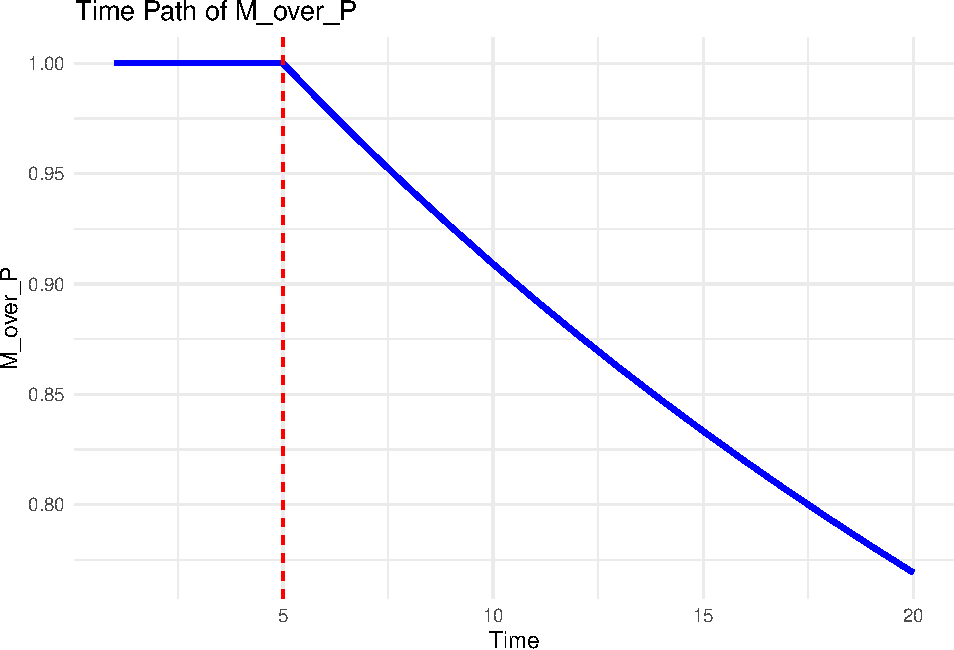
\includegraphics[keepaspectratio]{ProblemSet1_files/figure-latex/unnamed-chunk-20-5.pdf}}

\subsection{Problem 13(a) Temporary Decrease in U.S. Real Money
Demand}\label{problem-13a-temporary-decrease-in-u.s.-real-money-demand}

\textbf{Short-run effect (Point B):}

\begin{itemize}
\tightlist
\item
  \textbf{Money market:}\\
  A decline in real money demand shifts the \textbf{money demand curve
  left}, leading to a \textbf{temporary excess supply} of money at
  initial interest rates.

  \begin{itemize}
  \tightlist
  \item
    Result: \textbf{U.S. interest rates fall}
  \end{itemize}
\item
  \textbf{FX market:}

  \begin{itemize}
  \tightlist
  \item
    Lower \(i_{\$}\) makes dollar assets less attractive → capital
    outflows
  \item
    Dollar \textbf{depreciates} → \(E_{\$/€}\) \textbf{rises}
  \end{itemize}
\end{itemize}

\textbf{Long-run effect (Point C):}

\begin{itemize}
\tightlist
\item
  Because the shock is \textbf{temporary}, real money demand returns to
  original level
\item
  Interest rates return to normal
\item
  Exchange rate returns to initial value
\item
  Prices remain \textbf{unchanged}
\end{itemize}

\textbf{Summary (temporary):} - \textbf{Short run:}
\(i_{\$} \downarrow\), \(E_{\$/€} \uparrow\) - \textbf{Long run:} all
variables return to \textbf{initial equilibrium}

\subsection{Problem 13(b) Permanent Decrease in U.S. Real Money
Demand}\label{problem-13b-permanent-decrease-in-u.s.-real-money-demand}

This case leads to \textbf{permanent adjustments}, including the
\textbf{price level}:

\textbf{Short-run effect (Point B):}

\begin{itemize}
\tightlist
\item
  Similar to temporary case:

  \begin{itemize}
  \tightlist
  \item
    \(i_{\$} \downarrow\)
  \item
    \(E_{\$/€} \uparrow\) (dollar depreciates)
  \item
    \textbf{Overshooting}: exchange rate rises \textbf{more than
    long-run value}
  \end{itemize}
\end{itemize}

\textbf{Long-run effect (Point C):}

\begin{itemize}
\tightlist
\item
  Real money demand is permanently lower
\item
  With fixed nominal money supply \(M_{\$}\), this implies:

  \begin{itemize}
  \tightlist
  \item
    \textbf{Price level must rise} to lower \(M/P\) and re-establish
    equilibrium
  \item
    Interest rate \(i_{\$}\) returns to initial value
  \item
    Exchange rate remains \textbf{permanently higher} (weaker dollar)
  \end{itemize}
\end{itemize}

\textbf{Summary (permanent):} - \textbf{Short run:}
\(i_{\$} \downarrow\), \(E_{\$/€} \uparrow \uparrow\) (overshooting) -
\textbf{Long run:} \(P_{\$} \uparrow\), \(E_{\$/€} \uparrow\),
\(i_{\$} \rightarrow \text{initial}\)

\subsection{Problem 13(c) Time Path of Key Variables (Permanent
Shock)}\label{problem-13c-time-path-of-key-variables-permanent-shock}

\begin{longtable}[]{@{}
  >{\raggedright\arraybackslash}p{(\linewidth - 6\tabcolsep) * \real{0.2973}}
  >{\raggedright\arraybackslash}p{(\linewidth - 6\tabcolsep) * \real{0.2703}}
  >{\raggedright\arraybackslash}p{(\linewidth - 6\tabcolsep) * \real{0.2568}}
  >{\raggedright\arraybackslash}p{(\linewidth - 6\tabcolsep) * \real{0.1757}}@{}}
\toprule\noalign{}
\begin{minipage}[b]{\linewidth}\raggedright
Variable
\end{minipage} & \begin{minipage}[b]{\linewidth}\raggedright
Short-Run Behavior
\end{minipage} & \begin{minipage}[b]{\linewidth}\raggedright
Long-Run Behavior
\end{minipage} & \begin{minipage}[b]{\linewidth}\raggedright
Explanation
\end{minipage} \\
\midrule\noalign{}
\endhead
\bottomrule\noalign{}
\endlastfoot
Nominal money supply \(M_{\$}\) & No change & No change & Assumed
constant \\
Price level \(P_{\$}\) & Sticky & \textbf{Increases} & Adjusts to lower
real money demand \\
Real money balances \(M/P\) & \textbf{Excess} & Returns to lower
equilibrium & Price rise absorbs money supply \\
Interest rate \(i_{\$}\) & \textbf{Falls} & Returns to original & Real
balances normalize \\
Exchange rate \(E_{\$/€}\) & \textbf{Overshoots up} & Settles higher &
Dollar depreciates short- and long-term \\
\end{longtable}

\begin{itemize}
\tightlist
\item
  A \textbf{temporary fall} in real money demand causes a
  \textbf{short-run depreciation} of the dollar, but no long-run effect.
\item
  A \textbf{permanent fall} causes:

  \begin{itemize}
  \tightlist
  \item
    Short-run \textbf{overshooting} (due to sticky prices)
  \item
    Long-run \textbf{higher price level} and \textbf{permanent dollar
    depreciation}
  \item
    Interest rates return to equilibrium only after price adjustment
  \end{itemize}
\end{itemize}

\section{Problem 14: Monetary Policy and the FX Market --- South Korea
\&
Japan}\label{problem-14-monetary-policy-and-the-fx-market-south-korea-japan}

\textbf{Exchange rate definition:}\\
\[
E_{\text{won}/¥} = \text{South Korean won per Japanese yen}
\] → An \textbf{increase} in \(E_{\text{won}/¥}\) means the
\textbf{Korean won depreciates} relative to the yen.

\pandocbounded{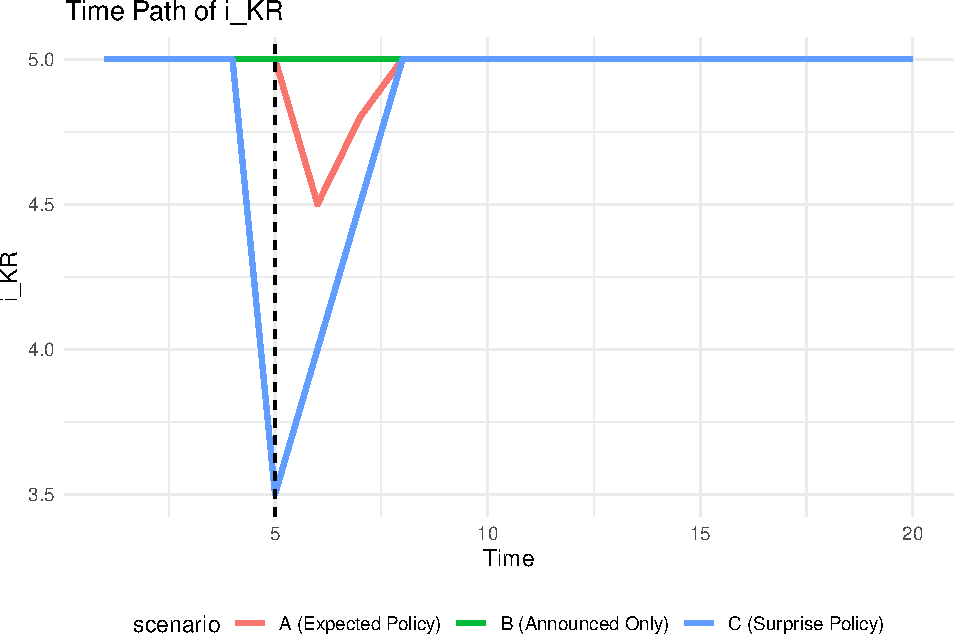
\includegraphics[keepaspectratio]{ProblemSet1_files/figure-latex/unnamed-chunk-21-1.pdf}}
\pandocbounded{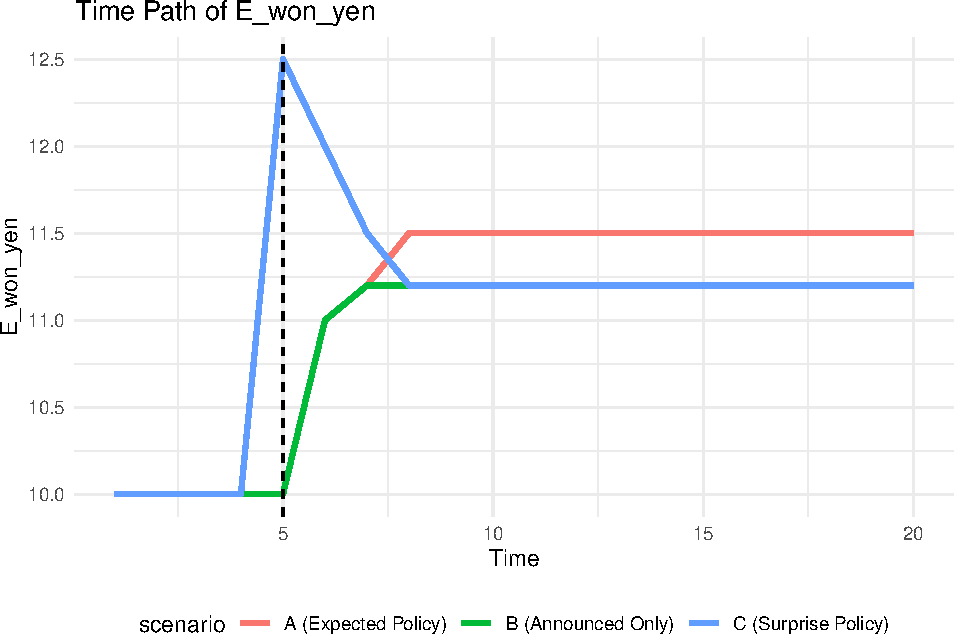
\includegraphics[keepaspectratio]{ProblemSet1_files/figure-latex/unnamed-chunk-21-2.pdf}}
\pandocbounded{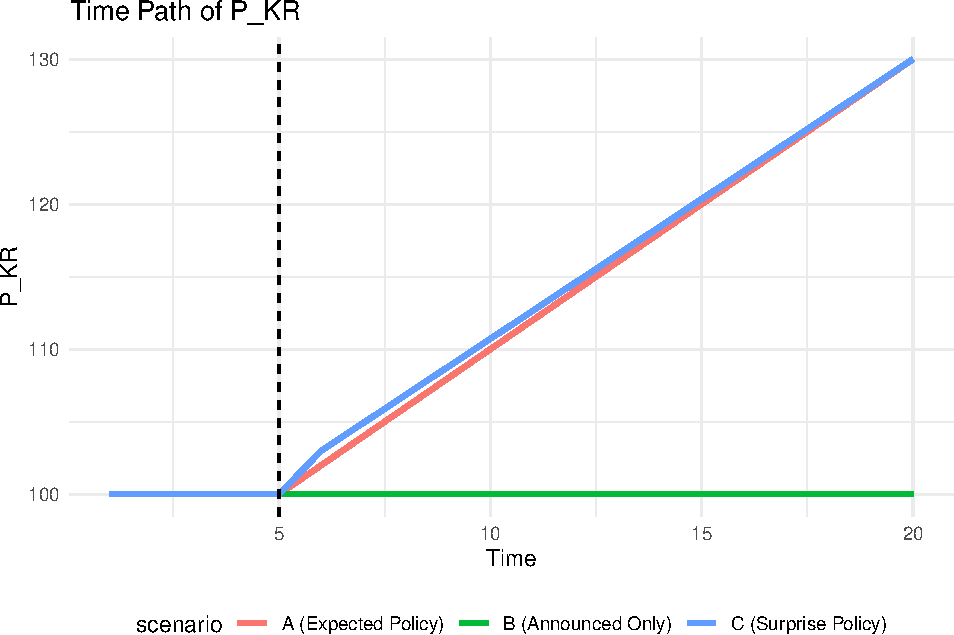
\includegraphics[keepaspectratio]{ProblemSet1_files/figure-latex/unnamed-chunk-21-3.pdf}}
\pandocbounded{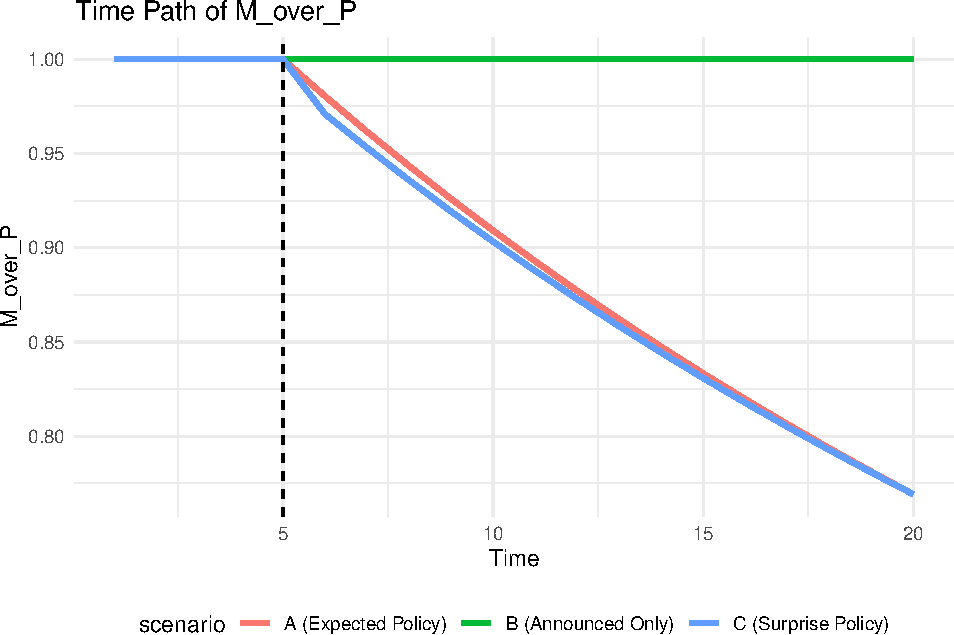
\includegraphics[keepaspectratio]{ProblemSet1_files/figure-latex/unnamed-chunk-21-4.pdf}}

\subsection{Problem 14(a) Permanent Increase in Korean Money
Supply}\label{problem-14a-permanent-increase-in-korean-money-supply}

\textbf{Short-run (Point B):}

\begin{itemize}
\tightlist
\item
  \textbf{Money Market:}

  \begin{itemize}
  \tightlist
  \item
    Bank of Korea increases nominal money supply → real money balances
    rise (prices sticky)
  \item
    \textbf{Korean interest rate falls} due to increased liquidity
  \end{itemize}
\item
  \textbf{FX Market:}

  \begin{itemize}
  \tightlist
  \item
    Lower interest rate in Korea → capital outflows
  \item
    \textbf{Won depreciates} → \(E_{\text{won}/¥}\) increases
  \end{itemize}
\end{itemize}

\textbf{Long-run (Point C):}

\begin{itemize}
\tightlist
\item
  Prices in Korea \textbf{rise}, reducing real money balances back to
  original
\item
  \textbf{Interest rate returns} to original level
\item
  Exchange rate remains \textbf{permanently higher} (permanent
  depreciation of won)
\end{itemize}

\textbf{Result:} - Short-run: won depreciates → Point B\\
- Long-run: higher price level and continued depreciation → Point C

\subsection{Problem 14(b) Announced but Unimplemented Policy (Believed
by
Investors)}\label{problem-14b-announced-but-unimplemented-policy-believed-by-investors}

\begin{itemize}
\tightlist
\item
  Investors \textbf{expect future money growth} → they expect future
  \textbf{inflation and depreciation}
\item
  Even though the policy isn't implemented, the \textbf{expected
  exchange rate \(E^e\)} rises
\item
  According to \textbf{Uncovered Interest Parity (UIP)}: \[
  i_{\text{KR}} \approx i_{\text{JP}} + \frac{E^e - E}{E}
  \] To satisfy UIP, the \textbf{current exchange rate
  \(E_{\text{won}/¥}\)} must \textbf{increase immediately}
\item
  Interest rates don't change (no actual monetary action)
\item
  The \textbf{won depreciates in the short run due to expectations}
\end{itemize}

\subsection{Problem 14(c) Unanticipated Permanent Increase in Money
Supply}\label{problem-14c-unanticipated-permanent-increase-in-money-supply}

\begin{itemize}
\tightlist
\item
  The policy is \textbf{not expected}, so markets don't price it in
  beforehand
\item
  Once implemented:

  \begin{itemize}
  \tightlist
  \item
    \textbf{Interest rate drops}
  \item
    \textbf{Won depreciates suddenly}
  \item
    Since there was no advance warning, \textbf{overshooting} occurs:

    \begin{itemize}
    \tightlist
    \item
      The exchange rate moves \textbf{more than its long-run value}
    \item
      Then adjusts back upward as prices rise
    \end{itemize}
  \end{itemize}
\end{itemize}

\subsection{Problem 14(d) Evaluating the
Statements}\label{problem-14d-evaluating-the-statements}

\subsubsection{\texorpdfstring{1. \emph{If a country wants to decrease
the value of its currency, it can do so (temporarily) without raising
domestic interest
rates.}}{1. If a country wants to decrease the value of its currency, it can do so (temporarily) without raising domestic interest rates.}}\label{if-a-country-wants-to-decrease-the-value-of-its-currency-it-can-do-so-temporarily-without-raising-domestic-interest-rates.}

\textbf{True}\\
A country can \textbf{decrease interest rates} via monetary expansion,
which \textbf{depreciates its currency} temporarily in the short run.

\subsubsection{\texorpdfstring{2. \emph{The central bank can increase
both the domestic price level and the value of its currency in the long
run.}}{2. The central bank can increase both the domestic price level and the value of its currency in the long run.}}\label{the-central-bank-can-increase-both-the-domestic-price-level-and-the-value-of-its-currency-in-the-long-run.}

\textbf{False}\\
In the long run, increasing the money supply \textbf{raises the domestic
price level} and leads to \textbf{currency depreciation}, not
appreciation.

\subsubsection{\texorpdfstring{3. \emph{The most effective way to
decrease the value of a currency is through surprising
investors.}}{3. The most effective way to decrease the value of a currency is through surprising investors.}}\label{the-most-effective-way-to-decrease-the-value-of-a-currency-is-through-surprising-investors.}

\textbf{True}\\
\textbf{Unanticipated policy} causes \textbf{exchange rate overshooting}
→ sudden, larger depreciation.\\
Surprises have stronger short-run effects than expected or announced
changes.

\textbf{Summary of Answers}

\begin{longtable}[]{@{}
  >{\raggedright\arraybackslash}p{(\linewidth - 2\tabcolsep) * \real{0.5294}}
  >{\raggedright\arraybackslash}p{(\linewidth - 2\tabcolsep) * \real{0.4706}}@{}}
\toprule\noalign{}
\begin{minipage}[b]{\linewidth}\raggedright
Scenario
\end{minipage} & \begin{minipage}[b]{\linewidth}\raggedright
FX Market Effect
\end{minipage} \\
\midrule\noalign{}
\endhead
\bottomrule\noalign{}
\endlastfoot
(a) Permanent M↑ (expected) & Short-run depreciation, long-run price ↑,
continued depreciation \\
(b) Announced M↑ (not implemented) & Short-run depreciation due to
expectations \\
(c) Surprise permanent M↑ & Sudden sharp depreciation (overshooting) \\
\end{longtable}

\end{document}
